%%%%%%%%%%%%%%%%
% Class
%%%%%%%%%%%%%%%%

	\documentclass[letterpaper,final]{article}
	
%%%%%%%%%%%%%%%%
% Packages
%%%%%%%%%%%%%%%%

	\usepackage{fancyhdr}
	\usepackage[margin=1in]{geometry}
	\usepackage{graphicx}
	\usepackage{amsmath}
	\usepackage{tikz}
		\usetikzlibrary{shapes}
%		\usetikzlibrary{decorations}
%		\usetikzlibrary{decorations.pathreplacing}
%		\usetikzlibrary{decorations.pathmorphing}

%%%%%%%%%%%%%%%%
% Other opts and styling
%%%%%%%%%%%%%%%%

	\graphicspath{{./assets/}}
	
	% Page headers
	\pagestyle{fancy}
	\renewcommand{\headrulewidth}{0pt}
	\fancyhead{}
	\fancyfoot{}
	\rhead{\thepage}
	
%%%%%%%%%%%%%%%%
% BEGIN DOCUMENT
%%%%%%%%%%%%%%%%

	\begin{document}

%%%%%%%%%%%%%%%%
% New commands
%%%%%%%%%%%%%%%%
	
	% Thick horizontal rule
	\newcommand{\HRule}{\rule{\linewidth}{0.5mm}}
	
	% Easy scientific notation
	\newcommand{\e}[1]{\ensuremath{\times 10^{#1}}}

%%%%%%%%%%%%%%%%
% TITLE PAGE
%%%%%%%%%%%%%%%%

	%!TEX root=./labNotes.tex

\begin{titlepage}
	{~ \\[5cm] }
	
	\noindent \HRule \\[0.4cm]
	{ \Huge \bfseries McDonald Lab \\[0.4cm] }
	{ \huge \bfseries Lab Protocols and Daily Log \\ }
	\HRule \\[0.4cm]
	
	\noindent { \Large Christopher Wetherill \\[0.15cm] }
	{ \large \emph{Virginia Polytechnic Institute and State University} }\\[11cm]
	
	\noindent Audit log available at https://github.com/faulconbridge/TBMH/tree/master/Virology
\end{titlepage}
		
%%%%%%%%%%%%%%%%
% CONTENTS
%%%%%%%%%%%%%%%%

	\part{Lab Protocols}
	%%%%%%%%%%
	% Protocol
	%%%%%%%%%%
	%!TEX root=./virology.tex

\section{Lab Protocols}

\subsection{Location of Common Materials}

\begin{tabular*}{\textwidth}{r | p{2in} p{2in}}
\hline
Item & Location & Storage \\
\hline
(In)complete Medium 199 & Incomplete Medium 199 is located in the cold room in the hallway immediately outside the lab. & Complete and serum-free Medium 199s are stored in the $4^{\circ}$C freezer in R2048.\\
Penicillin/Streptomycin Stock & P/S stock is located in the $-20^{\circ}$C freezer in the hallway immediately outside the lab. & Leftover stock is stored in the $4^{\circ}$C freezer in R2048.\\
L-Glutamine Stock & Stock is located in the $-20^{\circ}$C freezer in the hallway immediately outside the lab. & Leftover stock is stored in the $4^{\circ}$C freezer in R2048.\\
Amphotericin B stock & Stock is located in the $-20^{\circ}$C freezer in the hallway immediately outside the lab. & Leftover stock is stored in the $4^{\circ}$C freezer in R2048.\\
0.05\% Trypsin-EDTA & Stock is located in the $-20^{\circ}$C freezer in the hallway immediately outside the lab. & Leftover stock is stored in the $4^{\circ}$C freezer in R2048.\\
Trypsin ($2$mg/mL) & Stock is located in the $-20^{\circ}$ freezer in the hallway immediately outside the lab. & Leftover stock should be refrozen in a box labelled with your name.\\
Fetal Bovine Serum & Stock is located in the $-20^{\circ}$C freezer in the hallway immediately outside the lab. & Leftover stock is stored in the $4^{\circ}$C freezer in R2048.\\
(In)complete 2x EMEM & Stock is located in the cold room in the hallway immediately outside the lab. & Complete EMEM stock is stored in the $4^{\circ}$C freezer in R2048.\\
SeaPlaque Agarose & Stock is located in a jar above the benches immediately outside of the biosafety cabinet. & Leftover stock should be replaced where you found it.\\
10x PBS & Stock is located in a plastic bottle above the benches immediately outside of the biosafety cabinet. & Leftover stock should be replaced where you found it. \\
SA11 Stock & Stock is located in the $-20^{\circ}$ freezer in the hallway immediately outside the lab. & Leftover stock should be replaced where you found it.\\
Natural Red & Stock is located in the $4^{\circ}$ freezer in R2048. & Leftover stock should be replaced where you found it.\\
Lentiviral stock & Stock is located at the $-80^{\circ}$C freezer in the hallway immediately outside the lab. & Leftover stock should be replaced where you found it. \\
Polybreen & Stock is located in the $-20^{\circ}$C freezer in the hallway immediately outside the lab. & Leftover stock should be returned where you found it.\\
\hline
\end{tabular*}

\subsection{Recording Work and Labelling Materials}

All solutions should be labeled with your name, the date of preparation, and what the solution contains. All cell flasks should be labeled with your name, the date of preparation, the type of cell contained, and the passage of cell contained.

All work completed in the lab should be recorded in a laboratory notebook. Each page should contain entries from only a single day. The date of entry should be recorded at the top of each page. All writing must be easily readable and written in pen. Any errors should be struck through with a single solid line with the correction appearing next to it. Any space on a page not used at the end of a work day should be clearly crossed out in pen.

\subsection{Procedures for Autoclaving}

Ensure that all items have autoclave tape (if necessary). Place all items into the plastic bin found on the cart next to R2048. Take to the autoclave room. Add an autoclave quality indicator strip to the bin and insert into the autoclave. Close the door and select the appropriate options based on what is being sterilized. Start the cycle and fill out the autoclave use form on the bench next to the machine. Once the cycle is complete, retrieve the bin using the thick insulated gloves found in the lab (next to where the bin is stored). It is normal for there to be a small amount of water in the base of the bin.

\subsection{Preparation of Medium 199 (Serum-Free)}

{\bfseries Items Needed:}\footnote{The paper {\itshape Culturing, Storage, and Quantification of Rotaviruses} advises using different quantities of some materials below. Nonetheless, the following are the recommended quantities for use in lab.} \begin{enumerate}
	\item Incomplete Medium 199 ($500$mL)
	\item Penicillin/streptomycin stock ($5$mL)
	\item Amphotericin B stock ($1$mL; $250\mu$g/mL)
\end{enumerate}

In the biosafety cabinet, supplement $500$mL incomplete Medium 199 with $5$mL P/S stock and $1$mL amphotericin B stock. Store at $4^{\circ}$C for up to 3 months.

\subsection{Preparation of Medium 199 (Complete)}

{\bfseries Items Needed:}\footnote{See Note 1.} \begin{enumerate}
	\item Incomplete Medium 199 ($500$mL)
	\item Penicillin/streptomycin stock ($5$mL)
	\item Amphotericin B stock ($1$mL; $250\mu$g/mL)
	\item Fetal bovine serum ($55$mL)
\end{enumerate}

In the biosafety cabinet, supplement $500$mL incomplete Medium 199 with $5$mL P/S stock, $1$mL amphotericin B stock, and $55$mL fetal bovine serum. Store at $4^{\circ}$C for up to 3 months.

\subsection{Preparation of 1.2\% Agarose}

{\bfseries Items Needed:} \begin{enumerate}
	\item SeaPlaque agarose
	\item Milli-Q filtered water
\end{enumerate}

To a $500$mL flask add $1.2$g agarose for every $100$mL water. Inadvisable to fill flask to more than $400$mL. Cap and shake. Loosen lid. Apply autoclave tape to the lid. Autoclave approx. 20 min.

\subsection{Preparation of 2x EMEM (Serum-Free)}

{\bfseries Items Needed:} \begin{enumerate}
	\item incomplete 2x EMEM ($500$mL)
	\item $200$mM \textsc{l}-glutamine ($10$mL)
	\item P/S stock ($10$mL)
	\item $250\mu$g/ml amphotericin B stock ($1$mL)
\end{enumerate}

In the biosafety cabinet, to $500$mL incomplete 2x EMEM stock add $10$mL \textsc{L}-glutamine, $10$mL P/S stock, and $1$mL amphotericin B stock. Store at $4^{\circ}$C for up to 3 months.

\subsection{Preparation of PBS (Phosphate Buffered Saline)}

{\bfseries Items Needed:} \begin{enumerate}
	\item 10x PBS ($80$mL)
	\item milli-Q water ($720$mL)
\end{enumerate}

To a large graduated cylinder add $80$mL 10x PBS solution (use a $25$mL pipet). Fill the graduated cylinder to $800$mL with milli-Q-filtered water. Apply autoclave tape to the lid. Autoclave for 30 minutes.

\subsection{Procedure for Splitting MA104 Cells}

{\bfseries Items Needed:} \begin{enumerate}
	\item 1x PBS
	\item 0.05\% Trypsin-EDTA
	\item Complete Medium 199
	\item $150$cm$^2$ flask
\end{enumerate}

In a water bath, warm PBS, Trypsin, and complete Medium 199 to $37^{\circ}$C. Transfer all materials into the biosafety cabinet. Tilt the flask with your cells (having formed a confluent monolayer) such that the culture medium runs towards the neck of the flask. Vacuum out all culture medium using a small glass pipet inserted into the rubber vacuum hose. Dispose of the pipet. To the cell culture, add 10mL 1x PBS. Tilt the flask to ensure that all cells are thoroughly covered by PBS. Aspirate using a small glass pipet. Dispose of the pipet.

To the cell culture, add $5$mL Trypsin, tilting the flask forward and back to ensure that the cells are fully bathed. Vacuum out the Trypsin with a small glass pipet. Add a second $5$mL portion of Trypsin to the cell culture. Incubate at $37^{\circ}$C until all cells have detached from the surface and are free-floating. Lightly tap the flask with your hand if any cells remain attached.

To the cell culture add $15$mL complete Medium 199. (If you used less trypsin in the previous step, adjust the amount of Medium 199 applied such that there is $20$mL solution in the flask.)

To each new flask that you wish to prepare, add complete Medium 199 such that the final flask volume after the cell mixture is added will be equal to $25$mL. To determine the volume of cell mixture to add to each new flask, we use Table 1.1.

\begin{figure}[htp]
{\bfseries Table 1.1}\\[0.1cm]
\begin{tabular*}{\textwidth}{c c}
\hline
Cell dilution ratio & Cell mix volume to add \\
\hline
1:2 & 10mL \\
1:4 & 5mL \\
1:8 & 2.5mL \\
\hline
\end{tabular*}\\[0.1cm]
{\small {\itshape Note.} For example, if we wished to prepare one 1:4 dilution and two 1:8 dilutions, to our first flask we would add $15$mL complete Medium 199 and 10mL cell mixture; to each of our second two flasks we would add $20$mL complete Medium 199 and $5$mL cell mixture.}
\end{figure}

Cap the new flask(s) and tilt forward and back to evenly spread the cells. Loosen the lids and incubate at $37^{\circ}$C.

\subsection{Procedure for Plating MA104 Cells}

{\bfseries Items Needed:} \begin{enumerate}
	\item 1x PBS
	\item 0.05\% Trypsin
	\item Complete Medium 199
	\item Trypan Blue
	\item 6-well plates (x4)
\end{enumerate}

Aspirate the cell culture medium from the flask. Wash the cell monolayer in $10$mL $1x$ PBS and aspirate from the flask. Wash the cell monolayer in 5mL trypsin and aspirate from the flask. Bathe the cell monolayer in 5mL trypsin and incubate at $37^{\circ}$C until all cells have detached from the flask. (Check every 2 minutes.) Tap the flask with your hand to detach any remaining cells.

To the flask add $15$mL complete Medium 199 and mix thoroughly with the pipet. On a piece of parafilm, combine $10\mu$L cell mixture and $10\mu$L trypan blue. Mix thoroughly with a pipet. To a slide, add $20\mu$L such that the slide is completely filled with liquid. Insert into the automatic cell counter and record the result (total cells; live cells; percent alive). Use this to extrapolate the number of cells in the T150 flask and in each well as follow:

\begin{align*}
\frac{\text{cells}}{20\text{mL flask}} &= \frac{\text{cells}}{\text{mL}}\cdot \frac{20\text{mL}}{\text{flask}}\\
\frac{\text{cells}}{75\text{mL conical vial}} &= \left(\frac{1}{2}\cdot\frac{\text{cells}}{\text{flask}}\right)/\frac{75\text{mL}}{\text{conical vial}}\\
\frac{\text{cells}}{\text{well}} &= \frac{\text{cells}}{75\text{mL}}\cdot\frac{3\text{mL}}{\text{well}}
\end{align*}

To a $100$mL conical vial add $65$mL complete Medium 199. Supplement this with $10$mL cell solution. (These values may be doubled if 8 plates are being prepared. A T75 flask can accommodate 4 6-well plates; a T150 flask 8 6-well plates.) Transfer the fell mix to each of the wells, adding $3$mL cell solution per well. Spread the cells by tilting forward and back. Incubate the plates at $37^{\circ}$C for several days.

\subsection{Procedure for activating RV SA11 and Infecting MA104 Cells}

{\bfseries Items Needed:} \begin{enumerate}
	\item SA11 stock
	\item Trypsin (2mg/mL)
	\item Serum-free Medium 199
	\item 2x EMEM
	\item 1.2\% agarose
\end{enumerate}

In a large Eppie tube combine $400\mu$L rotavirus SA11 stock and $2\mu$L trypsin. Cap and incubate in a $37^{\circ}$C water bath for 1 hour. To each of 8 15mL plastic tubes add $2.7$mL serum-free Medium 199.

Add $300\mu$L virus mix to the first tube and label as $10^{-1}$. Mix the solution by vertex to homogenize. Take $300\mu$L of the $10^{-1}$ solution and add to the second tube. Label $10^{-2}$, cap, and mix by vertex. Repeat this process across the remaining tubes, ending with a viral concentration of $10^{-8}$. Store in the $4^{\circ}$C freezer if the cells are not going to be immediately infected. This is enough for 2 6-well plates. (Quantities may be increased proportionately if more than 2 plates are being infected at once.)

To 2 6-well plates, add the rotavirus titers. Each titer is to be performed in duplicate. To achieve this, add $\sim 1$mL of the $10^{-8}$ titer to two wells, then $10^{-7}$ titer to two wells, and so on. You will end with two plates as follow:

\begin{center}
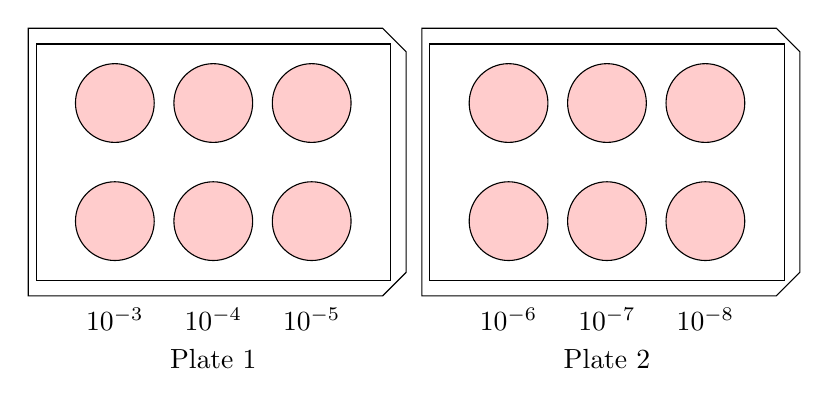
\begin{tikzpicture}

% Plate 1
\draw (0, 0) rectangle (4.5, 3);
\draw (-0.1, -0.2) -- (4.4, -0.2) -- (4.7, 0.1) -- (4.7, 2.9) -- (4.4, 3.2) -- (-0.1, 3.2) -- cycle;

% Wells
\draw [fill=red!20] (1, 0.75) circle (0.5);
\draw [fill=red!20] (1, 2.25) circle (0.5);
\node at (1,-0.5) {$10^{-3}$};

\draw [fill=red!20] (2.25, 0.75) circle (0.5);
\draw [fill=red!20] (2.25, 2.25) circle (0.5);
\node at (2.25,-0.5) {$10^{-4}$};

\draw [fill=red!20] (3.5, 0.75) circle (0.5);
\draw [fill=red!20] (3.5, 2.25) circle (0.5);
\node at (3.5,-0.5) {$10^{-5}$};

\node at (2.25, -1) {Plate 1};

% Plate 2
\draw (5, 0) rectangle (9.5, 3);
\draw (4.9, -0.2) -- (9.4, -0.2) -- (9.7, 0.1) -- (9.7, 2.9) -- (9.4, 3.2) -- (4.9, 3.2) -- cycle;

% Wells
\draw [fill=red!20] (6, 0.75) circle (0.5);
\draw [fill=red!20] (6, 2.25) circle (0.5);
\node at (6,-0.5) {$10^{-6}$};

\draw [fill=red!20] (7.25, 0.75) circle (0.5);
\draw [fill=red!20] (7.25, 2.25) circle (0.5);
\node at (7.25,-0.5) {$10^{-7}$};

\draw [fill=red!20] (8.5, 0.75) circle (0.5);
\draw [fill=red!20] (8.5, 2.25) circle (0.5);
\node at (8.5,-0.5) {$10^{-8}$};

\node at (7.25, -1) {Plate 2};

\end{tikzpicture}
\end{center}

Incubate the plates at $37^{\circ}$C for 1 hour.

Liquify a jar of $1.2\%$ agarose using a microwave. Warm 2x EMEM to $37^{\circ}$C in a water bath. For each plate infected, prepare a solution of 10mL agarose, 10mL 2x EMEM, and $5\mu$L trypsin. (Add the EMEM first, followed by the trypsin, followed by the agarose. Do not add trypsin to hot agarose.)

One plate at a time, aspirate the viral inoculant. (You may use a new pipet for each well or may use one pipet per plate, aspirating from the lowest concentration well to highest.) Quickly add to each well $\sim 3$mL of the agarose solution. Place the lid on the well and allow it to sit, undisturbed, for approximately 30 minutes (or until the agarose overlay has solidified). Incubate for several days at $37^{\circ}$C.

\subsection{Procedure for Performing RV Plaque Assay}

{\bfseries Items Needed:} \begin{enumerate}
	\item Neutral red
	\item 2x EMEM
	\item 1.2\% Agarose
\end{enumerate}

Liquefy 1.2\% agarose by microwave. For 4 6-well plates, mix $15$mL 2x EMEM, $15$mL 1.2\% agarose, and 1.5mL neutral red. Add $1$mL solution to each well and allow it to solidify. Incubate the plates at $37^{\circ}$C and count the plaques that have formed after $4-24$ hours of incubation.

\subsection{Procedure for Transducing MA104 Cells with siRNA-Expressing Lentiviral Vectors}

{\bfseries Items Needed:} \begin{enumerate}
	\item 1000x Polybreen
	\item Lentiviral vector
	\item Non-silencing vector (control)
	\item Complete M199
	\item 0.05\% Trypsin
	\item 1x PBS
	\item Trypan blue
\end{enumerate}

This procedure should be performed when the plated MA104 cells are $70-80\%$ confluent.

Select one well to use for a cell count. Aspirate the cell culture medium from this well. Add $1$mL PBS, spread evenly, and aspirate. Add $500\mu$L trypsin, spread evenly, and aspirate. Add $500\mu$L trypsin, spread evenly, and incubate the plate at $37{^\circ}$C until all cells have detached from the well.

To the well add $1.5$mL complete M199 and mix well. Take $10\mu$L cell mix and combine with $10\mu$L trypan blue. Apply this mixture to a slide and determine the number of cells per mL. Normalize this to the number of cells per well. (I.e., double the cell count per mL for the $2$mL cell soln in the target well.)

Calculate the dilution factor for the lentiviral vector by:
\begin{equation}
\left(\frac{\text{cells}}{\text{well}}\cdot \text{MOI}\right)/\left[\text{lentivirus}\right]
\end{equation}

For example, if there are $1.86\times 10^5$ cells per well, your original lentiviral concentration is $2.13\times 10^9$ particles per mL, and you want to transfect your cells with a multiplicity of infection (MOI) of $10$:
\begin{align*}
\text{dilution} &= \left(\frac{1.86\e{5}\text{ cells}}{\text{well}}\cdot \frac{10\text{ particles}}{1\text{ cell}}\right)/\frac{2.13\e{9}\text{ particles}}{\text{mL}} \\
&= \frac{1.86\e{6}\text{ particles}}{\text{well}}/\frac{2.13\e{9}\text{ particles}}{\text{mL}} \\
&= \frac{0.00087\text{mL}}{\text{well}} = \frac{0.87\mu\text{L}}{\text{well}}
\end{align*}

Per well, prepare a solution of $1$mL complete M199, $1\mu$L polybreen (diluted by a factor of $1000$), and the calculated volume of lentiviral vector. Repeat this procedure for the control NSV.

Aspirate the cell culture medium from each control and experimental well. To the experimental wells, add with one pipet $1$mL lentiviral solution to each well. To the control wells, add with a second pipet $1$mL control solution to each well. The final plates, using $5$ control and $5$ experimental wells, may look similar to the following:

\begin{center}
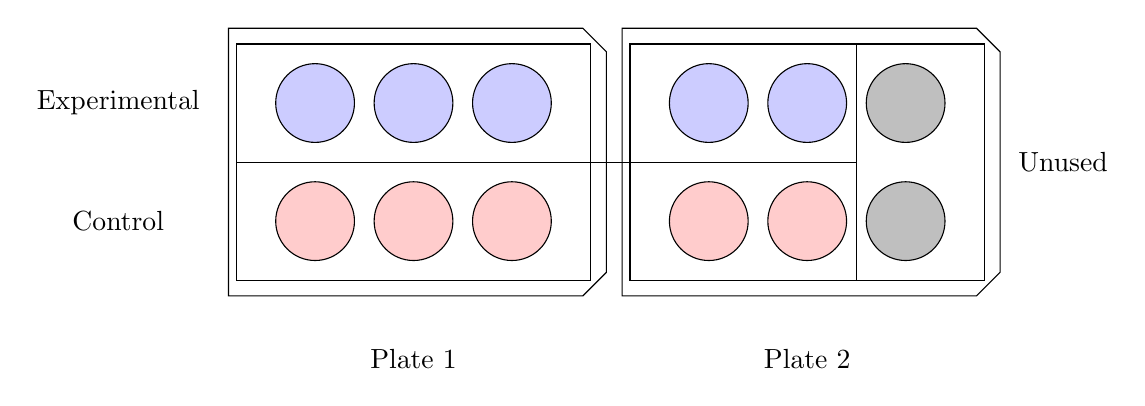
\begin{tikzpicture}

% Plate 1
\draw (0, 0) rectangle (4.5, 3);
\draw (-0.1, -0.2) -- (4.4, -0.2) -- (4.7, 0.1) -- (4.7, 2.9) -- (4.4, 3.2) -- (-0.1, 3.2) -- cycle;

% Wells
\draw [fill=red!20] (1, 0.75) circle (0.5);
\draw [fill=blue!20] (1, 2.25) circle (0.5);

\draw [fill=red!20] (2.25, 0.75) circle (0.5);
\draw [fill=blue!20] (2.25, 2.25) circle (0.5);

\draw [fill=red!20] (3.5, 0.75) circle (0.5);
\draw [fill=blue!20] (3.5, 2.25) circle (0.5);

\node at (2.25, -1) {Plate 1};

% Plate 2
\draw (5, 0) rectangle (9.5, 3);
\draw (4.9, -0.2) -- (9.4, -0.2) -- (9.7, 0.1) -- (9.7, 2.9) -- (9.4, 3.2) -- (4.9, 3.2) -- cycle;

% Wells
\draw [fill=red!20] (6, 0.75) circle (0.5);
\draw [fill=blue!20] (6, 2.25) circle (0.5);

\draw [fill=red!20] (7.25, 0.75) circle (0.5);
\draw [fill=blue!20] (7.25, 2.25) circle (0.5);

\draw [fill=gray!50] (8.5, 0.75) circle (0.5);
\draw [fill=gray!50] (8.5, 2.25) circle (0.5);

\node at (7.25, -1) {Plate 2};

\draw (0, 1.5) -- (7.875, 1.5);
\draw (7.875, 0) -- (7.875, 3);

\node [align = right] at (-1.5, 2.25) {Experimental};
\node [align = right] at (-1.5, 0.75) {Control};
\node at (10.5, 1.5) {Unused};
\end{tikzpicture}
\end{center}

Incubate these plates for 2 hours at $37^{\circ}$C. After 2 hours, add to each of the experimental wells $2$mL complete M199. Using a second pipet, add to each of the control wells $2$mL completeM199. The final volume of medium in each well should be $3$mL. Incubate for 48 hours at $37^{\circ}$C.

\subsection{Procedure for Infecting Cells Following Lentiviral Transduction}

\subsection{Procedure for Cell Count Following Infection of Lentivirally-Transduced Cells}

	\clearpage
	\part{Lab Notes}
	%%%%%%%%%%
	% August 2014
	%%%%%%%%%%
	%!TEX root=../labNotes.tex

\section{September 2014}

\subsection*{02 September 2014}

\begin{enumerate}
	\item Prepared serum-free Medium 199
		\begin{enumerate}
			\item Supplemented $500$mL incomplete Medium 199 (incomplete M199) with $5$mL penicillin/streptomycin stock ($100$U/mL penicillin; $100\mu$g/mL streptomycin final concentration) and $1$mL $250\mu$g/mL amphotericin B stock ($0.25\mu$g/mL amphotericin B final concentration)
			\item Stored at $4^{\circ}$C
		\end{enumerate}
	\item Prepared complete Medium 199
		\begin{enumerate}
				\item Supplemented $500$mL incomplete M199 with $5$mL penicillin/streptomycin stock ($100$U/mL penicillin; $100\mu$g/mL streptomycin final concentration) and $1$mL $250\mu$g/mL amphotericin B stock ($0.25\mu$g/mL amphotericin B final concentration), $55$mL fetal bovine serum
				\item Stored at $4^{\circ}$C
		\end{enumerate}
	\item MA104 cell split --- Passage 59
		\begin{enumerate}
			\item A T75 flask was split by Shu from her maintained stock, labeled, and incubated at $37^{\circ}$C
		\end{enumerate}
\end{enumerate}

\subsection*{03 September 2014}

\begin{enumerate}
	\item Prepared 2x EMEM, serum-free
		\begin{enumerate}
			\item Supplemented $500$mL 2x EMEM stock with $10$mL $200$mM L-glutamine stock ($4$mM L-glutamine final concentration), $10$mL penicillin/streptomycin stock ($200$U/mL penicillin; $200\mu$g/mL streptomycin final concentration), and $1$mL $250\mu$g/mL amphotericin B stock ($0.5\mu$g/mL amphotericin B final concentration)
			\item Stored at $4^{\circ}$C
		\end{enumerate}
	\item Prepared $400$mL $1.2$\% agarose
		\begin{enumerate}
			\item Combined $4.8020$g SeaPlaque agar to $\sim 400$mL milli-Q-filtered water
			\item Autoclaved for $20$ minutes
			\item Stored at room temperature
		\end{enumerate}
\end{enumerate}

	%%%%%%%%%%
	% September 2014
	%%%%%%%%%%
	%!TEX root=../virology.tex

\subsection*{09 September 2014}

\begin{enumerate}
	\item MA104 cell split --- Passage 60, from Passage 59, Flask A
		\begin{enumerate}
			\item Aspirated cell culture medium
			\item Rinsed cells in $10$mL 1x PBS; aspirated PBS
			\item Rinsed cells in $2$mL $0.05$\% trypsin; aspirated trypsin
			\item Bathed cells in $2$mL $0.05$\% trypsin
			\item Incubated cells at $37^{\circ}$C until all cells detached from flask
			\item Added $18$mL complete M199 to flask
			\item Added to $3$ T150 flasks $15$mL complete M199/$10$mL cell mix; $20$mL complete M199/$5$mL cell mix; and $20$mL complete M199/$5$mL cell mix. Respectively, flasks A, B, and C
			\item Gently shook flasks to distribute cells evenly
			\item Incubated at $37^{\circ}$C
		\end{enumerate}
\end{enumerate}

\subsection*{12 September 2014}

\begin{enumerate}
	\item Plated MA104 cells --- Passage 60, Flask A
		\begin{enumerate}
			\item Aspirated cell culture medium
			\item Rinsed cells in $10$mL 1x PBS; aspirated PBS
			\item Rinsed cells in $5$mL $0.05$\% trypsin; aspirated trypsin
			\item Bathed cells in $5$mL $0.05$\% trypsin
			\item Incubated cells at $37^{\circ}$C until all cells detached from flask
			\item Added $15$mL complete M199 to flask
			\item Took cell count by combining $10\mu$L cell mixture with $10\mu$L trypan blue:
			
				\begin{align*}
				\text{[cells]} &= \frac{3.91\e{5}\text{ cells}}{1\text{mL}} \\
				\frac{\text{cells}}{\text{flask}} &= \frac{3.91\e{5}\text{ cells}}{1\text{mL}} \cdot 20\text{mL} &= \frac{7.62\e{6}\text{ cells}}{20\text{mL}}\\
				\frac{\text{cells}}{10\text{mL cell mix}} &= \frac{7.62\e{6}\text{ cells}}{20\text{mL}}\cdot \frac{1}{2} &= \frac{3.81\e{6}\text{ cells}}{10\text{mL}}\\
				\frac{\text{cells}}{75\text{mL vial}} &= \frac{3.81\e{6}\text{ cells}}{75\text{mL}} &= \frac{5.08\e{4}\text{ cells}}{\text{mL}}\\
				\frac{\text{cells}}{3\text{mL well}} &= \frac{5.08\e{4}\text{ cells}}{\text{mL}} \cdot 3\text{mL} &= \frac{1.52\e{5}\text{ cells}}{\text{well}}\\
				\end{align*}
			\item Added $65$mL complete M199 and $10$mL cell mixture to $125$mL conical vial for final volume of $75$mL
			\item Transferred $3$mL solution to each well of 4 6-well plates
			\item Spread cells evenly by shaking
			\item Incubated at $37^{\circ}$C
		\end{enumerate}
\end{enumerate}
	%!TEX root=../virology.tex

\subsection*{15 September 2014}

\begin{enumerate}
	\item MA104 cell split --- Passage 61, from P60, Flask B
		\begin{enumerate}
			\item Aspirated cell culture medium
			\item Rinsed cells in $10$mL 1x PBS; aspirated PBS
			\item Rinsed cells in $5$mL $0.05$\% trypsin; aspirated trypsin
			\item Bathed cells in $5$mL $0.05$\% trypsin
			\item Incubated cells at $37^{\circ}$C until all cells detached from flask
			\item Added $15$mL complete M199 to flask
			\item Added to $3$ T150 flasks $20$mL complete M199/$5$mL cell mix; $22.5$mL complete M199/$2.5$mL cell mix; and $22.5$mL complete M199/$2.5$mL cell mix. Respectively, flasks A, B, and C
			\item Gently shook flasks to distribute cells evenly
			\item Incubated at $37^{\circ}$C
		\end{enumerate}
		
	\item Prepared 1x PBS
		\begin{enumerate}
			\item Combined $80$mL 10x PBS and $720$mL milli-Q-filtered water in a $1$L graduated cylinder
			\item Transferred to a $1$L bottle
			\item Autoclaved for 30 minutes
			\item Stored at room temperature
		\end{enumerate}
		
	\item Rotavirus activation and series dilution for P60A plated cells
		\begin{enumerate}
			\item Combined $400\mu$L SA11 rotavirus stock and $2$mL trypsin
			\item Incubated for 1 hour in a $37^{\circ}$C water bath
			\item Added $2.7$mL serum-free M199 to each of 8 $15$mL tubes
			\item To the first tube, added $300\mu$L rotavirus solution to a final concentration of $10^{-1}$
			\item Mixed contents by vertex
			\item To the next tube, added $300\mu$L rotavirus solution from the previous tube to a final concentration of $10^{-2}$
			\item Mixed contents by vertex
			\item Repeated serially for the remaining tubes ending with a concentration of $10^{-8}$ in the final tube
			\item Stored at $4^{\circ}$C
		\end{enumerate}
\end{enumerate}

\subsection*{16 September 2014}

\begin{enumerate}
	\item Plated MA104 cells --- Passage 60, Flask C
		\begin{enumerate}
			\item Aspirated cell culture medium
			\item Rinsed cells in $10$mL 1x PBS; aspirated PBS
			\item Rinsed cells in $5$mL $0.05$\% trypsin; aspirated trypsin
			\item Bathed cells in $5$mL $0.05$\% trypsin
			\item Incubated cells at $37^{\circ}$C until all cells detached from flask
			\item Added $15$mL complete M199 to flask
			\item Took cell count by combining $10\mu$L cell mixture with $10\mu$L trypan blue:
			
				\begin{align*}
				\text{[cells]} &= \frac{2.16\e{5}\text{ cells}}{1\text{mL}} \\
				\frac{\text{cells}}{\text{flask}} &= \frac{2.16\e{5}\text{ cells}}{1\text{mL}} \cdot 20\text{mL} &= \frac{4.32\e{6}\text{ cells}}{20\text{mL}}\\
				\frac{\text{cells}}{10\text{mL cell mix}} &= \frac{4.32\e{6}\text{ cells}}{20\text{mL}}\cdot \frac{1}{2} &= \frac{2.16\e{6}\text{ cells}}{10\text{mL}}\\
				\frac{\text{cells}}{75\text{mL vial}} &= \frac{2.16\e{6}\text{ cells}}{75\text{mL}} &= \frac{2.88\e{4}\text{ cells}}{\text{mL}}\\
				\frac{\text{cells}}{3\text{mL well}} &= \frac{2.88\e{4}\text{ cells}}{\text{mL}} \cdot 3\text{mL} &= \frac{8.64\e{4}\text{ cells}}{\text{well}}\\
				\end{align*}
			\item Added $65$mL complete M199 and $10$mL cell mixture to $125$mL conical vial for final volume of $75$mL
			\item Transferred $3$mL solution to each well of 4 6-well plates
			\item Spread cells evenly by shaking
			\item Incubated at $37^{\circ}$C
		\end{enumerate}
	\item Rotavirus infection of P60A plated cells
		\begin{enumerate}
			\item Washed monolayer in each well twice with serum-free M199 by dumping
			\item Added $\sim1$mL rotaviral solution to wells in concentrations from $10^{-3}$ to $10^{-8}$ with 2 wells being infected at each concentration of rotavirus
			\item Spread cells evenly by shaking
			\item Incubated at $37^{\circ}$C for 1 hour
		\end{enumerate}
	\item Agarose overlay of P60A plated cells
		\begin{enumerate}
			\item Liquefied 1.2\% agarose by microwave and equilibrated to $55^{\circ}$C
			\item For each plate of cells, prepared 1 vial of $10$mL agarose, $10$mL 2x EMEM, $5\mu$L $2$mg/mL trypsin
			\item Aspirated cell culture medium from each well
			\item To each well, added $\sim3$mL agarose solution
			\item Let agarose solidify
			\item Incubated at $37^{\circ}$C
		\end{enumerate}
\end{enumerate}

\subsection*{19 September 2014}

\begin{enumerate}
	\item MA104 cell split --- Passage 62, from Passage 61, Flask A
		\begin{enumerate}
			\item Aspirated cell culture medium
			\item Rinsed cells in $10$mL 1x PBS; aspirated PBS
			\item Rinsed cells in $5$mL $0.05$\% trypsin; aspirated trypsin
			\item Bathed cells in $5$mL $0.05$\% trypsin
			\item Incubated cells at $37^{\circ}$C until all cells detached from flask
			\item Added $15$mL complete M199 to flask
			\item Added to $3$ T150 flasks $20$mL complete M199/$5$mL cell mix; $22.5$mL complete M199/$2.5$mL cell mix; and $22.5$mL complete M199/$2.5$mL cell mix. Respectively, flasks A, B, and C
			\item Gently shook flasks to distribute cells evenly
			\item Incubated at $37^{\circ}$C
		\end{enumerate}
	\item Neutral red overlay of P60A plated cells
		\begin{enumerate}
			\item Prepared 2 vials, each with $7.5$mL 1.2\% agarose, $7.5$mL 2x EMEM, and $600\mu$L neutral red
			\item To each well of 2 6-well plates, added $\sim 1$mL prepared agarose solution (using 1 vial per plate)
			\item Let agarose solution solidify
			\item Incubated at $37^{\circ}$C for 4 hours
			\item Observed $3\e{6}$PFU/mL
		\end{enumerate}
\end{enumerate}
	%!TEX root=../virology.tex

\subsection*{21 September 2014}

\begin{enumerate}
	\item Rotavirus activation and series dilution for P60C plated cells
		\begin{enumerate}
			\item Combined $400\mu$L SA11 rotavirus stock and $2$mL trypsin
			\item Incubated for 1 hour in a $37^{\circ}$C water bath
			\item Added $2.7$mL serum-free M199 to each of 8 $15$mL tubes
			\item To the first tube, added $300\mu$L rotavirus solution to a final concentration of $10^{-1}$
			\item Mixed contents by vertex
			\item To the next tube, added $300\mu$L rotavirus solution from the previous tube to a final concentration of $10^{-2}$
			\item Mixed contents by vertex
			\item Repeated serially for the remaining tubes ending with a concentration of $10^{-8}$ in the final tube
			\item Stored at $4^{\circ}$C
		\end{enumerate}
\end{enumerate}

\subsection*{22 September 2014}

\begin{enumerate}
	\item Rotavirus infection of P60C plated cells
		\begin{enumerate}
			\item Washed monolayer in each well twice with serum-free M199 by dumping
			\item Added $\sim1$mL rotaviral solution to wells in concentrations from $10^{-3}$ to $10^{-8}$ with 2 wells being infected at each concentration of rotavirus
			\item Spread cells evenly by shaking
			\item Incubated at $37^{\circ}$C for 1 hour
		\end{enumerate}
	\item Agarose overlay of P60C plated cells
		\begin{enumerate}
			\item Liquefied 1.2\% agarose by microwave and equilibrated to $55^{\circ}$C
			\item For each plate of cells, prepared 1 vial of $10$mL agarose, $10$mL 2x EMEM, $5\mu$L $2$mg/mL trypsin
			\item Aspirated cell culture medium from each well
			\item To each well, added $\sim3$mL agarose solution
			\item Let agarose solidify
			\item Incubated at $37^{\circ}$C
		\end{enumerate}
\end{enumerate}

\subsection*{25 September 2014}

\begin{enumerate}
	\item Prepared complete Medium 199
		\begin{enumerate}
				\item Supplemented $500$mL incomplete M199 with $5$mL penicillin/streptomycin stock ($100$U/mL penicillin; $100\mu$g/mL streptomycin final concentration) and $1$mL $250\mu$g/mL amphotericin B stock ($0.25\mu$g/mL amphotericin B final concentration), $55$mL fetal bovine serum
				\item Stored at $4^{\circ}$C
		\end{enumerate}
	\item Plated MA104 cells --- Passage 61, Flask B
		\begin{enumerate}
			\item Aspirated cell culture medium
			\item Rinsed cells in $10$mL 1x PBS; aspirated PBS
			\item Rinsed cells in $5$mL $0.05$\% trypsin; aspirated trypsin
			\item Bathed cells in $5$mL $0.05$\% trypsin
			\item Incubated cells at $37^{\circ}$C until all cells detached from flask
			\item Added $15$mL complete M199 to flask
			\item Took cell count by combining $10\mu$L cell mixture with $10\mu$L trypan blue:
			
				\begin{align*}
				% Initial
				\text{[cells]} &= \frac{3.56\e{5}\text{ cells}}{1\text{mL}} \\
				% Cells / flask
				\frac{\text{cells}}{\text{flask}} &= \frac{3.56\e{5}\text{ cells}}{1\text{mL}} \cdot 20\text{mL} &= \frac{7.12\e{6}\text{ cells}}{20\text{mL}}\\
				% Cells / 10mL
				\frac{\text{cells}}{10\text{mL cell mix}} &= \frac{7.12\e{6}\text{ cells}}{20\text{mL}}\cdot \frac{1}{2} &= \frac{3.56\e{6}\text{ cells}}{10\text{mL}}\\
				% Cells / conical vial
				\frac{\text{cells}}{75\text{mL vial}} &= \frac{3.56\e{6}\text{ cells}}{75\text{mL}} &= \frac{4.75\e{4}\text{ cells}}{\text{mL}}\\
				% Cells / well
				\frac{\text{cells}}{3\text{mL well}} &= \frac{4.75\e{4}\text{ cells}}{\text{mL}} \cdot 3\text{mL} &= \frac{1.42\e{5}\text{ cells}}{\text{well}}\\
				\end{align*}
			\item Added $65$mL complete M199 and $10$mL cell mixture to $125$mL conical vial for final volume of $75$mL
			\item Transferred $3$mL solution to each well of 4 6-well plates
			\item Spread cells evenly by shaking
			\item Incubated at $37^{\circ}$C
		\end{enumerate}
	\item Neutral red overlay of P60C plated cells
		\begin{enumerate}
			\item Prepared 2 vials, each with $7.5$mL 1.2\% agarose, $7.5$mL 2x EMEM, and $600\mu$L neutral red
			\item To each well of 2 6-well plates, added $\sim 1$mL prepared agarose solution (using 1 vial per plate)
			\item Let agarose solution solidify
			\item Incubated at $37^{\circ}$C for 4 hours
			\item Agarose was applied too hot and plaques observed were not sufficient
		\end{enumerate}
\end{enumerate}

\subsection*{26 September 2014}

\begin{enumerate}
	\item Rotavirus activation and series dilution for P61B plated cells
		\begin{enumerate}
			\item Combined $400\mu$L SA11 rotavirus stock and $2$mL trypsin
			\item Incubated for 1 hour in a $37^{\circ}$C water bath
			\item Added $2.7$mL serum-free M199 to each of 8 $15$mL tubes
			\item To the first tube, added $300\mu$L rotavirus solution to a final concentration of $10^{-1}$
			\item Mixed contents by vertex
			\item To the next tube, added $300\mu$L rotavirus solution from the previous tube to a final concentration of $10^{-2}$
			\item Mixed contents by vertex
			\item Repeated serially for the remaining tubes ending with a concentration of $10^{-8}$ in the final tube
			\item Stored at $4^{\circ}$C
		\end{enumerate}
	\item MA104 cell split --- Passage 63, from Passage 62, Flask B
		\begin{enumerate}
			\item Aspirated cell culture medium
			\item Rinsed cells in $10$mL 1x PBS; aspirated PBS
			\item Rinsed cells in $5$mL $0.05$\% trypsin; aspirated trypsin
			\item Bathed cells in $5$mL $0.05$\% trypsin
			\item Incubated cells at $37^{\circ}$C until all cells detached from flask
			\item Added $15$mL complete M199 to flask
			\item Added to $3$ T150 flasks $22.5$mL complete M199/$2.5$mL cell mix; $22.5$mL complete M199/$2.5$mL cell mix; and $20$mL complete M199/$5$mL cell mix, respectively
			\item Gently shook flasks to distribute cells evenly
			\item Incubated at $37^{\circ}$C
		\end{enumerate}
\end{enumerate}
	%!TEX root=../labNotes.tex

\subsection*{28 September 2014}

\begin{enumerate}
	\item Rotavirus infection of P61B plated cells
		\begin{enumerate}
			\item Washed monolayer in each well twice with serum-free M199 by dumping
			\item Added $\sim 1$mL rotaviral solution to wells in concentrations from $10^{-3}$ to $10^{-8}$ with 2 wells being infected at each concentration of rotavirus
			\item Spread cells evenly by shaking
			\item Incubated at $37^{\circ}$C for 1 hour
		\end{enumerate}
	\item Agarose overlay of P61B plated cells
		\begin{enumerate}
			\item Liquefied 1.2\% agarose by microwave and equilibrated to $55^{\circ}$C
			\item For each plate of cells, prepared 1 vial of $10$mL agarose, $10$mL 2x EMEM, $5\mu$L $2$mg/mL trypsin
			\item Aspirated viral inoculant from each well
			\item To each well, added $\sim3$mL agarose solution
			\item Let agarose solidify
			\item Incubated at $37^{\circ}$C
		\end{enumerate}
	\item Plated MA104 cells --- Passage 62, Flask C
		\begin{enumerate}
			\item Aspirated cell culture medium
			\item Rinsed cells in $10$mL 1x PBS; aspirated PBS
			\item Rinsed cells in $5$mL $0.05$\% trypsin; aspirated trypsin
			\item Bathed cells in $5$mL $0.05$\% trypsin
			\item Incubated cells at $37^{\circ}$C until all cells detached from flask
			\item Added $15$mL complete M199 to flask
			\item Took cell count by combining $10\mu$L cell mixture with $10\mu$L trypan blue:
			
				\begin{align*}
				% Initial
				\text{[cells]} &= \frac{4.16\e{5}\text{ cells}}{1\text{mL}} \\
				% Cells / flask
				\frac{\text{cells}}{\text{flask}} &= \frac{4.16\e{5}\text{ cells}}{1\text{mL}} \cdot 20\text{mL} &= \frac{8.32\e{6}\text{ cells}}{20\text{mL}}\\
				% Cells / 10mL
				\frac{\text{cells}}{10\text{mL cell mix}} &= \frac{8.32\e{6}\text{ cells}}{20\text{mL}}\cdot \frac{1}{2} &= \frac{4.16\e{6}\text{ cells}}{10\text{mL}}\\
				% Cells / conical vial
				\frac{\text{cells}}{75\text{mL vial}} &= \frac{4.16\e{6}\text{ cells}}{75\text{mL}} &= \frac{5.55\e{4}\text{ cells}}{\text{mL}}\\
				% Cells / well
				\frac{\text{cells}}{3\text{mL well}} &= \frac{5.55\e{4}\text{ cells}}{\text{mL}} \cdot 3\text{mL} &= \frac{1.67\e{5}\text{ cells}}{\text{well}}\\
				\end{align*}
			\item Added $65$mL complete M199 and $10$mL cell mixture to $125$mL conical vial for final volume of $75$mL
			\item Transferred $3$mL solution to each well of 4 6-well plates
			\item Spread cells evenly by shaking
			\item Incubated at $37^{\circ}$C
		\end{enumerate}
\end{enumerate}

\subsection*{29 September 2014}

\begin{enumerate}
	\item Lentiviral transfection of P62C plated cells
		\begin{enumerate}
			\item Counted cells per well
				\begin{enumerate}
					\item To one well, added $1$mL 1x PBS; aspirated
					\item Rinsed in $500\mu$L trypsin; aspirated
					\item Bathed in $500\mu$L trypsin
					\item Incubated at $37^{\circ}$C until cells detached
					\item Added $1.5$mL complete M199
					\item Took cell count by combining $10\mu$L cell mixture with $10\mu$L trypan blue:
			
					\begin{align*}
					% Initial
					\text{[cells]} &= \frac{9.03\e{4}\text{ cells}}{1\text{mL}} \\
					% Cells / well
					\frac{\text{cells}}{2\text{mL well}} &= \frac{9.05\e{4}\text{ cells}}{\text{mL}} \cdot 2\text{mL} &= \frac{1.86\e{5}\text{ cells}}{\text{well}}\\
					\end{align*}
				\end{enumerate}
			\item Calculated RIO3 dilution
				\begin{align*}
					% initial
					\text{[RIO3]} &= \frac{2.13\e{9}\text{ particles}}{1\text{mL}}\\
					% MOI = 10
					\text{dilution}&= \left(\frac{1.86\e{5}\text{ cells}}{\text{well}}\cdot \frac{10\text{ particles}}{1\text{ cell}}\right)/\frac{2.13\e{9}\text{ particles}}{1\text{mL}}\\
					&= \frac{0.87\mu\text{L}}{\text{well}}\\
					&= \frac{4.4\mu\text{L}}{5\text{ wells}}
				\end{align*}
			\item Calculated NSV dilution
				\begin{align*}
					% initial
					\text{[NSV]} &= \frac{1.95\e{8}\text{ particles}}{1\text{mL}}\\
					% MOI = 10
					\text{dilution}&= \left(\frac{1.86\e{5}\text{ cells}}{\text{well}}\cdot \frac{10\text{ particles}}{1\text{ cell}}\right)/\frac{1.95\e{8}\text{ particles}}{1\text{mL}}\\
					&= \frac{9.54\mu\text{L}}{\text{well}}\\
					&= \frac{47.7\mu\text{L}}{5\text{ wells}}
				\end{align*}
			\item Prepared RIO3 wells
				\begin{enumerate}
					\item Combined $5$mL complete M199, $5\mu$L polybreen, and $4.4\mu$L RIO3 and mixed by vertex
					\item To each of the 5 experimental wells, added $1$mL RIO3 solution
					\item Spread evenly by gently shaking plates
				\end{enumerate}
			\item Prepared NSV control wells
				\begin{enumerate}
					\item Combined $5$mL complete M199, $5\mu$L polybreen, and $47.7\mu$L NSV and mixed by vertex
					\item To each of the 5 control wells, added $1$mL NSV solution
					\item Spread evenly by gently shaking plates
				\end{enumerate}
			\item Incubated plates at $37^{\circ}$C for 2 hours
			\item Supplemented each of the 5 experimental wells with an additional $2$mL complete M199 ($3$mL final well volume)
			\item With a separate pipet, supplemented each of the 5 control wells with an additional $2$mL complete M199 ($3$mL final well volume)
			\item Incubated plates at $37^{\circ}$C
		\end{enumerate}
\end{enumerate}

\section{October 2014}

\subsection*{01 October 2014}

\begin{enumerate}
	\item Prepared serum-free Medium 199
		\begin{enumerate}
			\item Supplemented $500$mL incomplete Medium 199 (incomplete M199) with $5$mL penicillin/streptomycin stock ($100$U/mL penicillin; $100\mu$g/mL streptomycin final concentration) and $1$mL $250\mu$g/mL amphotericin B stock ($0.25\mu$g/mL amphotericin B final concentration)
			\item Stored at $4^{\circ}$C
		\end{enumerate}
	\item Rotavirus infection of P62C plated cells (RIO3 and NSV transfected)
		\begin{enumerate}
			\item Counted cells per well
				\begin{enumerate}
					\item To one well, added $1$mL 1x PBS; aspirated
					\item Rinsed in $500\mu$L trypsin; aspirated
					\item Bathed in $500\mu$L trypsin
					\item Incubated at $37^{\circ}$C until cells detached
					\item Added $1.5$mL complete M199
					\item Took cell count by combining $10\mu$L cell mixture with $10\mu$L trypan blue:
			
					\begin{align*}
					% Initial
					\text{[cells]} &= \frac{1.18\e{5}\text{ cells}}{1\text{mL}} \\
					% Cells / well
					\frac{\text{cells}}{2\text{mL well}} &= \frac{1.18\e{5}\text{ cells}}{\text{mL}} \cdot 2\text{mL} &= \frac{2.36\e{5}\text{ cells}}{\text{well}}\\
					\end{align*}
				\end{enumerate}
			\item Calculated SA11 dilution
				\begin{align*}
					% initial
					\text{[SA11]} &= \frac{5\e{7}\text{ PFU}}{1\text{mL}}\\
					% MOI = 10
					\text{dilution}&= \left(\frac{2.36\e{5}\text{ cells}}{\text{well}}\cdot \frac{5\text{ particles}}{1\text{ cell}}\right)/\frac{5\e{7}\text{ PFU}}{1\text{mL}}\\
					&= \frac{23.6\mu\text{L}}{\text{well}}\\
					&= \frac{118\mu\text{L}}{5\text{ wells}}
				\end{align*}
			\item Prepared viral inoculant
				\begin{enumerate}
					\item To a vial, combined $400\mu$L SA11 and $2\mu$L trypsin
					\item Incubated in $37^{\circ}$C water bath for 1 hour
					\item Prepared vial of $10$mL serum-free M199
					\item Added to vial $236$mL viral solution (for infection of 10 wells)
				\end{enumerate}
			\item Washed wells twice with serum-free M199 by dumping
			\item Added to each well $1$mL viral solution
			\item Spread evenly by gently shaking plates
			\item Incubated plates at $37^{\circ}$C for 1 hour
			\item Aspirated viral inoculant from wells
			\item Added to each well $3$mL serum-free M199 and $0.75\mu$L trypsin
			\item Incubated plates at $37^{\circ}$C
		\end{enumerate}
	\item Plated MA104 cells --- Passage 63, Flask A
		%%%%%%%%%%%%%%%%%%%%%%%%%%%%%%
		% Go for a higher dilution --- these will be for more of
		% the *actual* exp runs, so we want 80% confluence
		% probably on Friday for LV transfection
		%%%%%%%%%%%%%%%%%%%%%%%%%%%%%%
		\begin{enumerate}
			\item Aspirated cell culture medium
			\item Rinsed cells in $10$mL 1x PBS; aspirated PBS
			\item Rinsed cells in $5$mL $0.05$\% trypsin; aspirated trypsin
			\item Bathed cells in $5$mL $0.05$\% trypsin
			\item Incubated cells at $37^{\circ}$C until all cells detached from flask
			\item Added $15$mL complete M199 to flask
			\item Took cell count by combining $10\mu$L cell mixture with $10\mu$L trypan blue:
			
				\begin{align*}
				% Initial
				\text{[cells]} &= \frac{4.61\e{5}\text{ cells}}{1\text{mL}} \\
				% Cells / flask
				\frac{\text{cells}}{\text{flask}} &= \frac{4.61\e{5}\text{ cells}}{1\text{mL}} \cdot 20\text{mL} &= \frac{9.22\e{6}\text{ cells}}{20\text{mL}}\\
				% Cells / 10mL
				\frac{\text{cells}}{10\text{mL cell mix}} &= \frac{9.22\e{6}\text{ cells}}{20\text{mL}}\cdot \frac{1}{2} &= \frac{4.61\e{6}\text{ cells}}{10\text{mL}}\\
				% Cells / conical vial
				\frac{\text{cells}}{75\text{mL vial}} &= \frac{4.61\e{6}\text{ cells}}{75\text{mL}} &= \frac{6.15\e{4}\text{ cells}}{\text{mL}}\\
				% Cells / well
				\frac{\text{cells}}{3\text{mL well}} &= \frac{6.15\e{4}\text{ cells}}{\text{mL}} \cdot 3\text{mL} &= \frac{1.84\e{5}\text{ cells}}{\text{well}}\\
				\end{align*}
			\item Added $65$mL complete M199 and $10$mL cell mixture to $125$mL conical vial for final volume of $75$mL
			\item Transferred $3$mL solution to each well of 4 6-well plates
			\item Spread cells evenly by shaking
			\item Incubated at $37^{\circ}$C
		\end{enumerate}
	\item Neutral red overlay of P62C plated cells
		\begin{enumerate}
			\item Prepared a vial with $7.5$mL 1.2\% agarose, $7.5$mL 2x EMEM, and $750\mu$L neutral red
			\item To each well of 2 6-well plates, added $\sim 1$mL prepared agarose solution
			\item Let agarose solution solidify
			\item Incubated at $37^{\circ}$C overnight
			\item Observed $\text{titer}=7\e{6}\text{ PFU/mL}$
		\end{enumerate}
\end{enumerate}

%%%%%%%%%%%%%%%%%%%%
% Thursday Plan
%%%%%%%%%%%%%%%%%%%%
% Probably split one flask (P63B),
% Bin the other (P63C)? Shoot for
% 3 1:8 dilutions so that there won't
% be much going on over the
% weekend, but we're good to get
% more runs in on Monday.
% Freeze transfected cells to lyse;
%%%%%%%%%%%%%%%%%%%%

\subsection*{02 October 2014}

\begin{enumerate}
	\item MA104 cell split --- Passage 64, from Passage 63, Flask B
		\begin{enumerate}
			\item Aspirated cell culture medium
			\item Rinsed cells in $10$mL 1x PBS; aspirated PBS
			\item Rinsed cells in $5$mL $0.05$\% trypsin; aspirated trypsin
			\item Bathed cells in $5$mL $0.05$\% trypsin
			\item Incubated cells at $37^{\circ}$C until all cells detached from flask
			\item Added $15$mL complete M199 to flask
			\item Added to $3$ T150 flasks $20$mL complete M199/$5$mL cell mix; $22.5$mL complete M199/$2.5$mL cell mix; and $22.5$mL complete M199/$2.5$mL cell mix. Respectively, flasks A, B, and C
			\item Gently shook flasks to distribute cells evenly
			\item Incubated at $37^{\circ}$C
		\end{enumerate}
	\item Lysed P62C transfected cells
		\begin{enumerate}
			\item Froze transfected cells in $-80^{\circ}$C freezer for 30 minutes; thawed
			\item Froze transfected cells in $-20^{\circ}$C freezer overnight
		\end{enumerate}
\end{enumerate}

%%%%%%%%%%%%%%%%%%%%
% Friday plan
%%%%%%%%%%%%%%%%%%%%
% Harvest RV from transfected cells
% Maybe infect plated cells?
%%%%%%%%%%%%%%%%%%%%

\subsection*{03 October 2014}

\begin{enumerate}
	\item Collected viral load from lysed P62C transfected cells
		\begin{enumerate}
			\item Thawed P62C cells
			\item Transferred content of each well to its own $15$mL tube
			\item Centrifuged tubes for 10 minutes at $500$RPM and $4^{\circ}$C
			\item Transfered supernatant from each centrifuged solution into fresh test tubes
			\item Stored at $-20^{\circ}$C
		\end{enumerate}
\end{enumerate}
	
	%%%%%%%%%%
	% October 2014
	%%%%%%%%%%
	%!TEX root=../virology.tex

\subsection*{06 October 2014}

\begin{enumerate}
	\item RIO3 Rotavirus activation and series dilution for P63A plated cells
		\begin{enumerate}
			\item Combined $400\mu$L SA11 reclaimed from RIO3-transfected cells (vial 3 of 5) and $2\mu$L trypsin
			\item Incubated for 1 hour in a $37^{\circ}$C water bath
			\item Added $2.7$mL serum-free M199 to each of 8 $15$mL tubes
			\item To the first tube, added $300\mu$L rotavirus solution to a final concentration of $10^{-1}$
			\item Mixed contents by vertex
			\item To the next tube, added $300\mu$L rotavirus solution from the previous tube to a final concentration of $10^{-2}$
			\item Mixed contents by vertex
			\item Repeated serially for the remaining tubes ending with a concentration of $10^{-8}$ in the final tube
			\item Stored at $4^{\circ}$C
		\end{enumerate}
	\item RIO3 Rotavirus infection of P63A plated cells
		\begin{enumerate}
			\item Washed monolayer in each well of 2 6-well plates twice with serum-free M199 by dumping
			\item Added $\sim 1$mL rotaviral solution to wells in concentrations from $10^{-3}$ to $10^{-8}$ with 2 wells being infected at each concentration of rotavirus
			\item Spread cells evenly by shaking
			\item Incubated at $37^{\circ}$C for 1 hour
		\end{enumerate}
	\item NSV Rotavirus activation and series dilution for P63A plated cells
		\begin{enumerate}
			\item Combined $400\mu$L SA11 reclaimed from NSV-transfected cells (vial 4 of 5) and $2\mu$L trypsin
			\item Incubated for 1 hour in a $37^{\circ}$C water bath
			\item Added $2.7$mL serum-free M199 to each of 8 $15$mL tubes
			\item To the first tube, added $300\mu$L rotavirus solution to a final concentration of $10^{-1}$
			\item Mixed contents by vertex
			\item To the next tube, added $300\mu$L rotavirus solution from the previous tube to a final concentration of $10^{-2}$
			\item Mixed contents by vertex
			\item Repeated serially for the remaining tubes ending with a concentration of $10^{-8}$ in the final tube
			\item Stored at $4^{\circ}$C
		\end{enumerate}
	\item NSV Rotavirus infection of P63A plated cells
		\begin{enumerate}
			\item Washed monolayer in each well of 2 6-well plates twice with serum-free M199 by dumping
			\item Added $\sim 1$mL rotaviral solution to wells in concentrations from $10^{-3}$ to $10^{-8}$ with 2 wells being infected at each concentration of rotavirus
			\item Spread cells evenly by shaking
			\item Incubated at $37^{\circ}$C for 1 hour
		\end{enumerate}
	\item Agarose overlay of P63A plated cells
		\begin{enumerate}
			\item Liquefied 1.2\% agarose by microwave and equilibrated to $55^{\circ}$C
			\item For each plate of cells (4 total), prepared 1 vial of $10$mL agarose, $10$mL 2x EMEM, $5\mu$L $2$mg/mL trypsin
			\item Aspirated viral inoculant from each well
			\item To each well, added $\sim3$mL agarose solution
			\item Let agarose solidify
			\item Incubated at $37^{\circ}$C
		\end{enumerate}
\end{enumerate}

	%!TEX root=../labNotes.tex

\subsection*{12 October 2014}

\begin{enumerate}
	\item RIO3 and NSV rotavirus activation and series dilution
		\begin{enumerate}
			\item For each of four samples (NSV vial 3; NSV vial 5; RIO3, vial 4; RIO3, vial 5):
				\begin{enumerate}
					\item Combined $400\mu$L SA11 reclaimed from transfected cells and $2\mu$L trypsin
					\item Incubated for 1 hour in a $37^{\circ}$C water bath
					\item Added $2.7$mL serum-free M199 to each of 8 $15$mL tubes
					\item To the first tube, added $300\mu$L rotavirus solution to a final concentration of $10^{-1}$
					\item Mixed contents by vertex
					\item To the next tube, added $300\mu$L rotavirus solution from the previous tube to a final concentration of $10^{-2}$
					\item Mixed contents by vertex
					\item Repeated serially for the remaining tubes ending with a concentration of $10^{-8}$ in the final tube
					\item Stored at $4^{\circ}$C
				\end{enumerate}
			\item Ended with 24 total vials, 8 of each of the SA11 samples identified previously
		\end{enumerate}
\end{enumerate}

\subsection*{13 October 2014}

\begin{enumerate}
	\item Rotavirus infection of P64B plated cells
		\begin{enumerate}
			\item For each of four samples (NSV vial 3; NSV vial 5; RIO3, vial 4; RIO3, vial 5):
				\begin{enumerate}
					\item Washed monolayer in each well of 2 6-well plates twice with serum-free M199 by dumping
					\item Added $\sim 1$mL rotaviral solution to wells in concentrations from $10^{-3}$ to $10^{-8}$ with 2 wells being infected at each concentration of rotavirus
					\item Spread cells evenly by shaking
					\item Incubated at $37^{\circ}$C for 1 hour
				\end{enumerate}
		\end{enumerate}
	\item Agarose overlay of P64B plated cells
		\begin{enumerate}
			\item For each of four samples (NSV vial 3; NSV vial 5; RIO3, vial 4; RIO3, vial 5):
				\begin{enumerate}
					\item Liquefied 1.2\% agarose by microwave and equilibrated to $55^{\circ}$C
					\item For each plate of cells (8 total), prepared 1 vial of $10$mL agarose, $10$mL 2x EMEM, $5\mu$L $2$mg/mL trypsin
					\item Aspirated viral inoculant from each well
					\item To each well, added $\sim3$mL agarose solution
					\item Let agarose solidify
					\item Incubated at $37^{\circ}$C
				\end{enumerate}
			\item Ended with 8 infected 6-well plates with 2 infected plates (viral titers from $10^{-3}-10^{-8}$ in duplicate) for each of the 4 viral samples
		\end{enumerate}
\end{enumerate}

\subsection*{14 October 2014}

\begin{enumerate}
	\item Plated MA104 cells --- Passage 65, Flask A
		\begin{enumerate}
			\item Aspirated cell culture medium
			\item Rinsed cells in $10$mL 1x PBS; aspirated PBS
			\item Rinsed cells in $5$mL $0.05$\% trypsin; aspirated trypsin
			\item Bathed cells in $5$mL $0.05$\% trypsin
			\item Incubated cells at $37^{\circ}$C until all cells detached from flask
			\item Added $15$mL complete M199 to flask
			\item Took cell count by combining $10\mu$L cell mixture with $10\mu$L trypan blue:
			
				\begin{align*}
				% Initial
				\text{[cells]} &= \frac{2.31\e{5}\text{ cells}}{1\text{mL}} \\
				% Cells / flask
				\frac{\text{cells}}{\text{flask}} &= \frac{2.31\e{5}\text{ cells}}{1\text{mL}} \cdot 20\text{mL} &= \frac{4.62\e{6}\text{ cells}}{20\text{mL}}\\
				% Cells / conical vial
				\frac{\text{cells}}{150\text{mL vial}} &= \frac{4.62\e{6}\text{ cells}}{150\text{mL}} &= \frac{3.08\e{4}\text{ cells}}{\text{mL}}\\
				% Cells / well
				\frac{\text{cells}}{3\text{mL well}} &= \frac{3.08\e{4}\text{ cells}}{\text{mL}} \cdot 3\text{mL} &= \frac{9.24\e{4}\text{ cells}}{\text{well}}\\
				\end{align*}
			\item Added $130$mL complete M199 and $20$mL cell mixture to $250$mL conical vial for final volume of $150$mL
			\item Transferred $3$mL solution to each well of 8 6-well plates
			\item Spread cells evenly by shaking
			\item Incubated at $37^{\circ}$C
		\end{enumerate}
\end{enumerate}

%%%%%%%%%%%%%%%%%%%%
% Wednesday Plan
%%%%%%%%%%%%%%%%%%%%
% Plate P65B for new transfection?
% 
% Might need to split P65C or D
%%%%%%%%%%%%%%%%%%%%

\subsection*{15 October 2014}

\begin{enumerate}
	\item RIO3 and NSV rotavirus activation and series dilution
		\begin{enumerate}
			\item For each of four samples (NSV vial 1; NSV vial 2; RIO3, vial 1; RIO3, vial 2):
				\begin{enumerate}
					\item Combined $400\mu$L SA11 reclaimed from transfected cells and $2\mu$L trypsin
					\item Incubated for 1 hour in a $37^{\circ}$C water bath
					\item Added $2.7$mL serum-free M199 to each of 8 $15$mL tubes
					\item To the first tube, added $300\mu$L rotavirus solution to a final concentration of $10^{-1}$
					\item Mixed contents by vertex
					\item To the next tube, added $300\mu$L rotavirus solution from the previous tube to a final concentration of $10^{-2}$
					\item Mixed contents by vertex
					\item Repeated serially for the remaining tubes ending with a concentration of $10^{-8}$ in the final tube
					\item Stored at $4^{\circ}$C
				\end{enumerate}
			\item Ended with 24 total vials, 8 of each of the SA11 samples identified previously
		\end{enumerate}
\end{enumerate}

%%%%%%%%%%%%%%%%%%%%
% Thursday Plan
%%%%%%%%%%%%%%%%%%%%
% Split P65C/D if not already
%
% Neutral red staining of P64B
% plated cells
% 
% If confluent, infect P65A plated
% cells with NSV/RIO 1 and 2
%%%%%%%%%%%%%%%%%%%%

\subsection*{16 October 2014}

\begin{enumerate}
	\item Plated MA104 cells --- Passage 65, Flask C
		\begin{enumerate}
			\item Aspirated cell culture medium
			\item Rinsed cells in $10$mL 1x PBS; aspirated PBS
			\item Rinsed cells in $5$mL $0.05$\% trypsin; aspirated trypsin
			\item Bathed cells in $5$mL $0.05$\% trypsin
			\item Incubated cells at $37^{\circ}$C until all cells detached from flask
			\item Added $15$mL complete M199 to flask
			\item Took cell count by combining $10\mu$L cell mixture with $10\mu$L trypan blue:
			
				\begin{align*}
				% Initial
				\text{[cells]} &= \frac{2.46\e{5}\text{ cells}}{1\text{mL}} \\
				% Cells / flask
				\frac{\text{cells}}{\text{flask}} &= \frac{2.46\e{5}\text{ cells}}{1\text{mL}} \cdot 20\text{mL} &= \frac{4.92\e{6}\text{ cells}}{20\text{mL}}\\
				% Cells / 5mL sample
				\frac{\text{cells}}{5\text{mL sample}} &= \frac{4.92\e{6}\text{ cells}}{20\text{mL}}\cdot \frac{1}{4} &= \frac{1.23\e{6}\text{ cells}}{5\text{mL}}\\
				% Cells / conical vial
				\frac{\text{cells}}{37.5\text{mL vial}} &= \frac{1.23\e{6}\text{ cells}}{37.5\text{mL}} &= \frac{3.28\e{4}\text{ cells}}{\text{mL}}\\
				% Cells / well
				\frac{\text{cells}}{3\text{mL well}} &= \frac{3.28\e{4}\text{ cells}}{\text{mL}} \cdot 3\text{mL} &= \frac{9.84\e{4}\text{ cells}}{\text{well}}\\
				\end{align*}
			\item Added $32.5$mL complete M199 and $5$mL cell mixture to $125$mL conical vial for final volume of $150$mL
			\item Transferred $3$mL solution to each well of 2 6-well plates
			\item Spread cells evenly by shaking
			\item Incubated at $37^{\circ}$C for 1 hour and then transferred to $31^{\circ}$C incubator
		\end{enumerate}
	\item MA104 cell split --- Passage 66, from Passage 65, Flask D
		\begin{enumerate}
			\item Aspirated cell culture medium
			\item Rinsed cells in $10$mL 1x PBS; aspirated PBS
			\item Rinsed cells in $5$mL $0.05$\% trypsin; aspirated trypsin
			\item Bathed cells in $5$mL $0.05$\% trypsin
			\item Incubated cells at $37^{\circ}$C until all cells detached from flask
			\item Added $15$mL complete M199 to flask
			\item Added to $4$ T150 flasks $20$mL complete M199/$5$mL cell mix; $22.5$mL complete M199/$2.5$mL cell mix; and $22.5$mL complete M199/$2.5$mL cell mix. Respectively, flasks A, B, and C
			\item Gently shook flasks to distribute cells evenly
			\item Incubated at $37^{\circ}$C
		\end{enumerate}
	\item Neutral red overlay of P64B plated cells (RIO3, vial 4)
		\begin{enumerate}
			\item Prepared a vial with $7.5$mL 1.2\% agarose, $7.5$mL 2x EMEM, and $750\mu$L neutral red
			\item To each well of 2 6-well plates, added $\sim 1$mL prepared agarose solution
			\item Let agarose solution solidify
			\item Incubated at $37^{\circ}$C overnight
			\item Observed $\text{titer}=x\e{6}\text{ PFU/mL}$
		\end{enumerate}
	\item Neutral red overlay of P64B plated cells (RIO3, vial 5)
		\begin{enumerate}
			\item Procedure was identical to above
			\item Observed $\text{titer}=x\e{6}\text{ PFU/mL}$
		\end{enumerate}
	\item Neutral red overlay of P64B plated cells (NSV, vial 3)
		\begin{enumerate}
			\item Procedure was identical to above
			\item Observed $\text{titer}=x\e{6}\text{ PFU/mL}$
		\end{enumerate}
	\item Neutral red overlay of P64B plated cells (NSV, vial 5)
		\begin{enumerate}
			\item Procedure was identical to above
			\item Observed $\text{titer}=x\e{6}\text{ PFU/mL}$
		\end{enumerate}
\end{enumerate}

%%%%%%%%%%%%%%%%%%%%
% Friday Plan
%%%%%%%%%%%%%%%%%%%%
% If not plated Thurs, infect P65A
% plated cells with NSV/RIO 1, 2
%%%%%%%%%%%%%%%%%%%%

%	\item Rotavirus infection of P65A plated cells
%		\begin{enumerate}
%			\item For each of four samples (NSV vial 1; NSV vial 2; RIO3, vial 1; RIO3, vial 2):
%				\begin{enumerate}
%					\item Washed monolayer in each well of 2 6-well plates twice with serum-free M199 by dumping
%					\item Added $\sim 1$mL rotaviral solution to wells in concentrations from $10^{-3}$ to $10^{-8}$ with 2 wells being infected at each concentration of rotavirus
%					\item Spread cells evenly by shaking
%					\item Incubated at $37^{\circ}$C for 1 hour
%				\end{enumerate}
%		\end{enumerate}
%	\item Agarose overlay of P65A plated cells
%		\begin{enumerate}
%			\item For each of four samples (NSV vial 1; NSV vial 2; RIO3, vial 1; RIO3, vial 2):
%				\begin{enumerate}
%					\item Liquefied 1.2\% agarose by microwave and equilibrated to $55^{\circ}$C
%					\item For each plate of cells (8 total), prepared 1 vial of $10$mL agarose, $10$mL 2x EMEM, $5\mu$L $2$mg/mL trypsin
%					\item Aspirated viral inoculant from each well
%					\item To each well, added $\sim3$mL agarose solution
%					\item Let agarose solidify
%					\item Incubated at $37^{\circ}$C
%				\end{enumerate}
%			\item Ended with 8 infected 6-well plates with 2 infected plates (viral titers from $10^{-3}-10^{-8}$ in duplicate) for each of the 4 viral samples
%		\end{enumerate}

	%!TEX root=../labNotes.tex

\subsection*{20 October 2014}

\begin{enumerate}
	% Ended up having no use for these...
	\item Disposed of P65C plated cells.
	
	\item Prepared complete Medium 199
		\begin{enumerate}
				\item Supplemented $500$mL incomplete M199 with $5$mL penicillin/streptomycin stock ($100$U/mL penicillin; $100\mu$g/mL streptomycin final concentration) and $1$mL $250\mu$g/mL amphotericin B stock ($0.25\mu$g/mL amphotericin B final concentration), $55$mL fetal bovine serum
				\item Stored at $4^{\circ}$C
		\end{enumerate}
	\item Prepared serum-free Medium 199
		\begin{enumerate}
			\item Supplemented $500$mL incomplete M199 with $5$mL penicillin/streptomycin stock ($100$U/mL penicillin; $100\mu$g/mL streptomycin final concentration) and $1$mL $250\mu$g/mL amphotericin B stock ($0.25\mu$g/mL amphotericin B final concentration)
			\item Stored at $4^{\circ}$C
		\end{enumerate}

	% These will all be plated (24 plates total) on Friday
	% for infection with SA11 collected from transduced cells
	\item MA104 cell split --- Passage 67, from Passage 66, Flask A
		\begin{enumerate}
			\item Aspirated cell culture medium
			\item Rinsed cells in $10$mL 1x PBS; aspirated PBS
			\item Rinsed cells in $5$mL $0.05$\% trypsin; aspirated trypsin
			\item Bathed cells in $5$mL $0.05$\% trypsin
			\item Incubated cells at $37^{\circ}$C until all cells detached from flask
			\item Added $15$mL complete M199 to flask
			\item Added to $3$ T150 flasks $20$mL complete M199/$5$mL cell mix; $20$mL complete M199/$5$mL cell mix; and $20$mL complete M199/$5$mL cell mix. Respectively, flasks A, B, and C
			\item Gently shook flasks to distribute cells evenly
			\item Incubated at $37^{\circ}$C
		\end{enumerate}
	
	% These cells will all be transduced with a lentiviral vector
	% to produce samples of virus from all 12 target kinases
	\item Plated MA104 cells --- Passage 66, Flask B
		\begin{enumerate}
			\item Aspirated cell culture medium
			\item Rinsed cells in $10$mL 1x PBS; aspirated PBS
			\item Rinsed cells in $5$mL $0.05$\% trypsin; aspirated trypsin
			\item Bathed cells in $5$mL $0.05$\% trypsin
			\item Incubated cells at $37^{\circ}$C until all cells detached from flask
			\item Added $15$mL complete M199 to flask
			\item Took cell count by combining $10\mu$L cell mixture with $10\mu$L trypan blue:
			
				\begin{align*}
				% Initial
				\text{[cells]} &= \frac{2.41\e{5}\text{ cells}}{1\text{mL}} \\
				% Cells / flask
				\frac{\text{cells}}{\text{flask}} &= \frac{2.41\e{5}\text{ cells}}{1\text{mL}} \cdot 20\text{mL} &= \frac{4.82\e{6}\text{ cells}}{20\text{mL}}\\
				% Cells / conical vial
				\frac{\text{cells}}{150\text{mL vial}} &= \frac{4.82\e{6}\text{ cells}}{150\text{mL}} &= \frac{3.28\e{4}\text{ cells}}{\text{mL}}\\
				% Cells / well
				\frac{\text{cells}}{3\text{mL well}} &= \frac{3.21\e{4}\text{ cells}}{\text{mL}} \cdot 3\text{mL} &= \frac{9.63\e{4}\text{ cells}}{\text{well}}\\
				\end{align*}
			\item Added $120$mL complete M199 and $20$mL cell mixture to $250$mL conical vial for final volume of $150$mL
			\item Transferred $3$mL solution to each well of 8 6-well plates
			\item Spread cells evenly by shaking
			\item Incubated at $37^{\circ}$C for 1 hour and then transferred to $31^{\circ}$C incubator
		\end{enumerate}
\end{enumerate}

\subsection*{21 October 2014}

\begin{enumerate}
	\item Neutral red overlay of P64B plated cells (RIO3, vial 1)
		\begin{enumerate}
			\item Prepared a vial with $7.5$mL 1.2\% agarose, $7.5$mL 2x EMEM, and $750\mu$L neutral red
			\item To each well of 2 6-well plates, added $\sim 1$mL prepared agarose solution
			\item Let agarose solution solidify
			\item Incubated at $37^{\circ}$C overnight
			\item Observed $\text{titer}=1.5\e{8}\text{ PFU/mL}$
		\end{enumerate}
	\item Neutral red overlay of P64B plated cells (RIO3, vial 2)
		\begin{enumerate}
			\item Procedure was identical to above
			\item Observed $\text{titer}=1\e{8}\text{ PFU/mL}$
		\end{enumerate}
	\item Neutral red overlay of P64B plated cells (NSV, vial 1)
		\begin{enumerate}
			\item Procedure was identical to above
			\item Observed $\text{titer}=2.5\e{8}\text{ PFU/mL}$
		\end{enumerate}
	\item Neutral red overlay of P64B plated cells (NSV, vial 2)
		\begin{enumerate}
			\item Procedure was identical to above
			\item Observed $\text{titer}=2\e{8}\text{ PFU/mL}$
		\end{enumerate}
	\item Prepared $400$mL $1.2$\% agarose
		\begin{enumerate}
			\item Combined $4.8106$g SeaPlaque agar to $\sim 400$mL milli-Q-filtered water
			\item Autoclaved for $20$ minutes
			\item Stored at room temperature
		\end{enumerate}
\end{enumerate}


\subsection*{22 October 2014}
%%%%%%%%%%%%%%%%%%%%%%%%%%%%%%%%%%%%%%%%
% BEGIN LENTIVIRAL TRANSDUCTION
%%%%%%%%%%%%%%%%%%%%%%%%%%%%%%%%%%%%%%%%
\begin{enumerate}
	\item Lentiviral transduction of P66B plated cells
		\begin{enumerate}
			\item Counted cells per well
				\begin{enumerate}
					\item To one well, added $1$mL 1x PBS; aspirated
					\item Rinsed in $500\mu$L trypsin; aspirated
					\item Bathed in $500\mu$L trypsin
					\item Incubated at $37^{\circ}$C until cells detached
					\item Added $1.5$mL complete M199
					\item Took cell count by combining $10\mu$L cell mixture with $10\mu$L trypan blue:
			
					\begin{align*}
					% Initial
					\text{[cells]} &= \frac{1.00\e{5}\text{ cells}}{1\text{mL}} \\
					% Cells / well
					\frac{\text{cells}}{2\text{mL well}} &= \frac{1.00\e{5}\text{ cells}}{\text{mL}} \cdot 2\text{mL} &= \frac{2.00\e{5}\text{ cells}}{\text{well}}\\
					\end{align*}
				\end{enumerate}
%%%%%%%%%%%%%%%%%%%%%%%%%%%%%%%%%%%%%%%%
% CALCULATE DILUTIONS OF KINASES
%%%%%%%%%%%%%%%%%%%%%%%%%%%%%%%%%%%%%%%%
			\item Calculation of kinase dilutions
				\begin{enumerate}
				\item Calculated NSV dilution
						\begin{align*}
							% initial
							\text{[NSV]} &= \frac{1.95\e{8}\text{ particles}}{1\text{mL}}\\
							% MOI = 10
							\text{dilution}&= \left(\frac{2.00\e{5}\text{ cells}}{\text{well}}\cdot \frac{10\text{ particles}}{1\text{ cell}}\right)/\frac{1.95\e{8}\text{ particles}}{1\text{mL}}\\
							&= \frac{10.3\mu\text{L}}{\text{well}}\\
							&= \frac{30.8\mu\text{L}}{3\text{ wells}}
						\end{align*}
					\item Calculated RIO3 dilution
						\begin{align*}
							% initial
							\text{[RIO3]} &= \frac{2.13\e{9}\text{ particles}}{1\text{mL}}\\
							% MOI = 10
							\text{dilution}&= \left(\frac{2.00\e{5}\text{ cells}}{\text{well}}\cdot \frac{10\text{ particles}}{1\text{ cell}}\right)/\frac{2.13\e{9}\text{ particles}}{1\text{mL}}\\
							&= \frac{0.939\mu\text{L}}{\text{well}}\\
							&= \frac{2.82\mu\text{L}}{5\text{ wells}}
						\end{align*}
					\item Calculated GUCY2D dilution
						\begin{align*}
							% initial
							\text{[GUCY2D]} &= \frac{2.43\e{9}\text{ particles}}{1\text{mL}}\\
							% MOI = 10
							\text{dilution}&= \left(\frac{2.00\e{5}\text{ cells}}{\text{well}}\cdot \frac{10\text{ particles}}{1\text{ cell}}\right)/\frac{2.43\e{9}\text{ particles}}{1\text{mL}}\\
							&= \frac{0.823\mu\text{L}}{\text{well}}\\
							&= \frac{2.47\mu\text{L}}{3\text{ wells}}
						\end{align*}
					\item Calculated CSNK2B dilution
							\begin{align*}
							% initial
							\text{[CSNK2B]} &= \frac{1.77\e{9}\text{ particles}}{1\text{mL}}\\
							% MOI = 10
							\text{dilution}&= \left(\frac{2.00\e{5}\text{ cells}}{\text{well}}\cdot \frac{10\text{ particles}}{1\text{ cell}}\right)/\frac{1.77\e{9}\text{ particles}}{1\text{mL}}\\
							&= \frac{1.13\mu\text{L}}{\text{well}}\\
							&= \frac{3.39\mu\text{L}}{3\text{ wells}}
						\end{align*}
					\item Calculated EPHA1 dilution
							\begin{align*}
							% initial
							\text{[EPHA1]} &= \frac{3.59\e{9}\text{ particles}}{1\text{mL}}\\
							% MOI = 10
							\text{dilution}&= \left(\frac{2.00\e{5}\text{ cells}}{\text{well}}\cdot \frac{10\text{ particles}}{1\text{ cell}}\right)/\frac{3.59\e{9}\text{ particles}}{1\text{mL}}\\
							&= \frac{0.557\mu\text{L}}{\text{well}}\\
							&= \frac{1.67\mu\text{L}}{3\text{ wells}}
						\end{align*}
					\item Calculated ZMYND8 dilution
							\begin{align*}
							% initial
							\text{[ZMYND8]} &= \frac{3.42\e{9}\text{ particles}}{1\text{mL}}\\
							% MOI = 10
							\text{dilution}&= \left(\frac{2.00\e{5}\text{ cells}}{\text{well}}\cdot \frac{10\text{ particles}}{1\text{ cell}}\right)/\frac{3.42\e{9}\text{ particles}}{1\text{mL}}\\
							&= \frac{0.585\mu\text{L}}{\text{well}}\\
							&= \frac{1.75\mu\text{L}}{3\text{ wells}}
						\end{align*}
					\item Calculated CKM dilution
							\begin{align*}
							% initial
							\text{[CKM]} &= \frac{2.38\e{9}\text{ particles}}{1\text{mL}}\\
							% MOI = 10
							\text{dilution}&= \left(\frac{2.00\e{5}\text{ cells}}{\text{well}}\cdot \frac{10\text{ particles}}{1\text{ cell}}\right)/\frac{2.38\e{9}\text{ particles}}{1\text{mL}}\\
							&= \frac{0.840\mu\text{L}}{\text{well}}\\
							&= \frac{2.52\mu\text{L}}{3\text{ wells}}
						\end{align*}
					\item Calculated PIK3CA dilution
							\begin{align*}
							% initial
							\text{[PIK3CA]} &= \frac{1.04\e{9}\text{ particles}}{1\text{mL}}\\
							% MOI = 10
							\text{dilution}&= \left(\frac{2.00\e{5}\text{ cells}}{\text{well}}\cdot \frac{10\text{ particles}}{1\text{ cell}}\right)/\frac{1.04\e{9}\text{ particles}}{1\text{mL}}\\
							&= \frac{1.92\mu\text{L}}{\text{well}}\\
							&= \frac{5.77\mu\text{L}}{3\text{ wells}}
						\end{align*}
					\item Calculated STK11IP dilution
							\begin{align*}
							% initial
							\text{[STK11IP]} &= \frac{3.66\e{9}\text{ particles}}{1\text{mL}}\\
							% MOI = 10
							\text{dilution}&= \left(\frac{2.00\e{5}\text{ cells}}{\text{well}}\cdot \frac{10\text{ particles}}{1\text{ cell}}\right)/\frac{3.66\e{9}\text{ particles}}{1\text{mL}}\\
							&= \frac{0.546\mu\text{L}}{\text{well}}\\
							&= \frac{1.64\mu\text{L}}{3\text{ wells}}
						\end{align*}
					\item Calculated SKAP1 dilution
							\begin{align*}
							% initial
							\text{[SKAP1]} &= \frac{2.79\e{9}\text{ particles}}{1\text{mL}}\\
							% MOI = 10
							\text{dilution}&= \left(\frac{2.00\e{5}\text{ cells}}{\text{well}}\cdot \frac{10\text{ particles}}{1\text{ cell}}\right)/\frac{2.79\e{9}\text{ particles}}{1\text{mL}}\\
							&= \frac{0.717\mu\text{L}}{\text{well}}\\
							&= \frac{2.15\mu\text{L}}{3\text{ wells}}
						\end{align*}
					\item Calculated UCK2 dilution
							\begin{align*}
							% initial
							\text{[UCK2]} &= \frac{2.35\e{9}\text{ particles}}{1\text{mL}}\\
							% MOI = 10
							\text{dilution}&= \left(\frac{2.00\e{5}\text{ cells}}{\text{well}}\cdot \frac{10\text{ particles}}{1\text{ cell}}\right)/\frac{2.35\e{9}\text{ particles}}{1\text{mL}}\\
							&= \frac{0.851\mu\text{L}}{\text{well}}\\
							&= \frac{2.55\mu\text{L}}{3\text{ wells}}
						\end{align*}
					\item Calculated TGF-$\alpha$ dilution
							\begin{align*}
							% initial
							\text{[TGF-$\alpha$]} &= \frac{1.50\e{8}\text{ particles}}{1\text{mL}}\\
							% MOI = 10
							\text{dilution}&= \left(\frac{2.00\e{5}\text{ cells}}{\text{well}}\cdot \frac{10\text{ particles}}{1\text{ cell}}\right)/\frac{1.50\e{8}\text{ particles}}{1\text{mL}}\\
							&= \frac{13.3\mu\text{L}}{\text{well}}\\
							&= \frac{40.0\mu\text{L}}{3\text{ wells}}
						\end{align*}
				\end{enumerate}
%%%%%%%%%%%%%%%%%%%%%%%%%%%%%%%%%%%%%%%%
% PREPARE LV SOLNS AND TRANSFECT CELLS
%%%%%%%%%%%%%%%%%%%%%%%%%%%%%%%%%%%%%%%%
			\item Lentiviral transduction of wells
				\begin{enumerate}
					\item Prepared NSV control wells
						\begin{enumerate}
							\item Combined $3$mL complete M199, $3\mu$L polybrene, and $30.8\mu$L NSV and mixed by vertex
							\item Aspirated cell culture medium from wells
							\item To each of the 3 wells, added $1$mL NSV solution
							\item Spread evenly by gently shaking plates
						\end{enumerate}
					\item Prepared RIO3 wells
						\begin{enumerate}
							\item Combined $3$mL complete M199, $3\mu$L polybrene, and $2.82\mu$L RIO3 and mixed by vertex
							\item Aspirated cell culture medium from wells
							\item To each of the 3 wells, added $1$mL RIO3 solution
							\item Spread evenly by gently shaking plates
						\end{enumerate}
					\item Prepared GUCY2D wells
						\begin{enumerate}
							\item Combined $3$mL complete M199, $3\mu$L polybrene, and $2.47\mu$L GUCY2D and mixed by vertex
							\item Aspirated cell culture medium from wells
							\item To each of the 3 wells, added $1$mL RIO3 solution
							\item Spread evenly by gently shaking plates
						\end{enumerate}
					\item Prepared CSNK2B wells
						\begin{enumerate}
							\item Combined $3$mL complete M199, $3\mu$L polybrene, and $3.39\mu$L CSNK2B and mixed by vertex
							\item Aspirated cell culture medium from wells
							\item To each of the 3 wells, added $1$mL NSV solution
							\item Spread evenly by gently shaking plates
						\end{enumerate}
					\item Prepared EPHA1 wells
						\begin{enumerate}
							\item Combined $3$mL complete M199, $3\mu$L polybrene, and $1.67\mu$L EPHA1 and mixed by vertex
							\item Aspirated cell culture medium from wells
							\item To each of the 3 wells, added $1$mL RIO3 solution
							\item Spread evenly by gently shaking plates
						\end{enumerate}
					\item Prepared ZMYND8 wells
						\begin{enumerate}
							\item Combined $3$mL complete M199, $3\mu$L polybrene, and $1.75\mu$L ZMYND8 and mixed by vertex
							\item Aspirated cell culture medium from wells
							\item To each of the 3 wells, added $1$mL NSV solution
							\item Spread evenly by gently shaking plates
						\end{enumerate}
					\item Prepared CKM wells
						\begin{enumerate}
							\item Combined $3$mL complete M199, $3\mu$L polybrene, and $2.52\mu$L CKM and mixed by vertex
							\item Aspirated cell culture medium from wells
							\item To each of the 3 wells, added $1$mL RIO3 solution
							\item Spread evenly by gently shaking plates
						\end{enumerate}
					\item Prepared PIK3CA wells
						\begin{enumerate}
							\item Combined $3$mL complete M199, $3\mu$L polybrene, and $5.77\mu$L PIK3CA and mixed by vertex
							\item Aspirated cell culture medium from wells
							\item To each of the 3 wells, added $1$mL NSV solution
							\item Spread evenly by gently shaking plates
						\end{enumerate}
					\item Prepared STK11IP wells
						\begin{enumerate}
							\item Combined $3$mL complete M199, $3\mu$L polybrene, and $1.64\mu$L STK11IP and mixed by vertex
							\item Aspirated cell culture medium from wells
							\item To each of the 3 wells, added $1$mL RIO3 solution
							\item Spread evenly by gently shaking plates
						\end{enumerate}
					\item Prepared SKAP1 wells
						\begin{enumerate}
							\item Combined $3$mL complete M199, $3\mu$L polybrene, and $2.15\mu$L SKAP1 and mixed by vertex
							\item Aspirated cell culture medium from wells
							\item To each of the 3 wells, added $1$mL NSV solution
							\item Spread evenly by gently shaking plates
						\end{enumerate}
					\item Prepared UCK2 wells
						\begin{enumerate}
							\item Combined $3$mL complete M199, $3\mu$L polybrene, and $2.55\mu$L UCK2 and mixed by vertex
							\item Aspirated cell culture medium from wells
							\item To each of the 3 wells, added $1$mL RIO3 solution
							\item Spread evenly by gently shaking plates
						\end{enumerate}
					\item Prepared TGF-$\alpha$ wells
						\begin{enumerate}
							\item Combined $3$mL complete M199, $3\mu$L polybrene, and $40.0\mu$L TGF-$\alpha$ and mixed by vertex
							\item Aspirated cell culture medium from wells
							\item To each of the 3 wells, added $1$mL NSV solution
							\item Spread evenly by gently shaking plates
						\end{enumerate}
				\end{enumerate}
			\item Incubated plates at $37^{\circ}$C for 2 hours
			\item Supplemented each of the wells with an additional $2$mL complete M199 ($3$mL final well volume)
			\item Incubated plates at $37^{\circ}$C for 48 hours
		\end{enumerate}
	\item MA104 cell split --- Passage 67-2, from Passage 66, Flask C
		\begin{enumerate}
			\item Aspirated cell culture medium
			\item Rinsed cells in $10$mL 1x PBS; aspirated PBS
			\item Rinsed cells in $5$mL $0.05$\% trypsin; aspirated trypsin
			\item Bathed cells in $5$mL $0.05$\% trypsin
			\item Incubated cells at $37^{\circ}$C until all cells detached from flask
			\item Added $15$mL complete M199 to flask
			\item Added to $3$ T150 flasks $20$mL complete M199/$5$mL cell mix; $20$mL complete M199/$5$mL cell mix; and $20$mL complete M199/$5$mL cell mix. Respectively, flasks A2, B2, and C2
			\item Gently shook flasks to distribute cells evenly
			\item Incubated at $37^{\circ}$C
		\end{enumerate}
\end{enumerate}

\subsection*{23 October 2014}

\begin{enumerate}
	\item Prepared complete Medium 199
		\begin{enumerate}
				\item Supplemented $500$mL incomplete M199 with $5$mL penicillin/streptomycin stock ($100$U/mL penicillin; $100\mu$g/mL streptomycin final concentration) and $1$mL $250\mu$g/mL amphotericin B stock ($0.25\mu$g/mL amphotericin B final concentration), $55$mL fetal bovine serum
				\item Stored at $4^{\circ}$C
		\end{enumerate}
	\item Prepared serum-free Medium 199
		\begin{enumerate}
			\item Supplemented $500$mL incomplete M199 with $5$mL penicillin/streptomycin stock ($100$U/mL penicillin; $100\mu$g/mL streptomycin final concentration) and $1$mL $250\mu$g/mL amphotericin B stock ($0.25\mu$g/mL amphotericin B final concentration)
			\item Stored at $4^{\circ}$C
		\end{enumerate}
		
	\item Plated MA104 cells --- Passage 67, Flask A
		\begin{enumerate}
			\item Aspirated cell culture medium
			\item Rinsed cells in $10$mL 1x PBS; aspirated PBS
			\item Rinsed cells in $5$mL $0.05$\% trypsin; aspirated trypsin
			\item Bathed cells in $5$mL $0.05$\% trypsin
			\item Incubated cells at $37^{\circ}$C until all cells detached from flask
			\item Added $15$mL complete M199 to flask
			\item Took cell count by combining $10\mu$L cell mixture with $10\mu$L trypan blue:
			
				\begin{align*}
				% Initial
				\text{[cells]} &= \frac{3.31\e{5}\text{ cells}}{1\text{mL}} \\
				% Cells / flask
				\frac{\text{cells}}{\text{flask}} &= \frac{3.31\e{5}\text{ cells}}{1\text{mL}} \cdot 20\text{mL} &= \frac{6.62\e{6}\text{ cells}}{20\text{mL}}\\
				% Cells / conical vial
				\frac{\text{cells}}{150\text{mL vial}} &= \frac{6.62\e{6}\text{ cells}}{150\text{mL}} &= \frac{4.41\e{4}\text{ cells}}{\text{mL}}\\
				% Cells / well
				\frac{\text{cells}}{3\text{mL well}} &= \frac{4.41\e{4}\text{ cells}}{\text{mL}} \cdot 3\text{mL} &= \frac{1.32\e{5}\text{ cells}}{\text{well}}\\
				\end{align*}
			\item Added $120$mL complete M199 and $20$mL cell mixture to $250$mL conical vial for final volume of $150$mL
			\item Transferred $3$mL solution to each well of 8 6-well plates
			\item Spread cells evenly by shaking
			\item Labeled plates A1--A8
			\item Incubated at $37^{\circ}$C for 1 hour and then transferred to $31^{\circ}$C incubator
		\end{enumerate}
	\item Plated MA104 cells --- Passage 67, Flask B
		\begin{enumerate}
			\item Aspirated cell culture medium
			\item Rinsed cells in $10$mL 1x PBS; aspirated PBS
			\item Rinsed cells in $5$mL $0.05$\% trypsin; aspirated trypsin
			\item Bathed cells in $5$mL $0.05$\% trypsin
			\item Incubated cells at $37^{\circ}$C until all cells detached from flask
			\item Added $15$mL complete M199 to flask
			\item Took cell count by combining $10\mu$L cell mixture with $10\mu$L trypan blue:
			
				\begin{align*}
				% Initial
				\text{[cells]} &= \frac{4.72\e{5}\text{ cells}}{1\text{mL}} \\
				% Cells / flask
				\frac{\text{cells}}{\text{flask}} &= \frac{4.72\e{5}\text{ cells}}{1\text{mL}} \cdot 20\text{mL} &= \frac{9.44\e{6}\text{ cells}}{20\text{mL}}\\
				% Cells / conical vial
				\frac{\text{cells}}{150\text{mL vial}} &= \frac{9.44\e{6}\text{ cells}}{150\text{mL}} &= \frac{6.29\e{4}\text{ cells}}{\text{mL}}\\
				% Cells / well
				\frac{\text{cells}}{3\text{mL well}} &= \frac{3.21\e{4}\text{ cells}}{\text{mL}} \cdot 3\text{mL} &= \frac{1.89\e{5}\text{ cells}}{\text{well}}\\
				\end{align*}
			\item Added $120$mL complete M199 and $20$mL cell mixture to $250$mL conical vial for final volume of $150$mL
			\item Transferred $3$mL solution to each well of 8 6-well plates
			\item Spread cells evenly by shaking
			\item Labeled plates B1--B8
			\item Incubated at $37^{\circ}$C for 1 hour and then transferred to $31^{\circ}$C incubator
		\end{enumerate}
	\item Plated MA104 cells --- Passage 67, Flask C
		\begin{enumerate}
			\item Aspirated cell culture medium
			\item Rinsed cells in $10$mL 1x PBS; aspirated PBS
			\item Rinsed cells in $5$mL $0.05$\% trypsin; aspirated trypsin
			\item Bathed cells in $5$mL $0.05$\% trypsin
			\item Incubated cells at $37^{\circ}$C until all cells detached from flask
			\item Added $15$mL complete M199 to flask
			\item Took cell count by combining $10\mu$L cell mixture with $10\mu$L trypan blue:
			
				\begin{align*}
				% Initial
				\text{[cells]} &= \frac{1.76\e{5}\text{ cells}}{1\text{mL}} \\
				% Cells / flask
				\frac{\text{cells}}{\text{flask}} &= \frac{1.76\e{5}\text{ cells}}{1\text{mL}} \cdot 20\text{mL} &= \frac{3.52\e{6}\text{ cells}}{20\text{mL}}\\
				% Cells / conical vial
				\frac{\text{cells}}{150\text{mL vial}} &= \frac{3.52\e{6}\text{ cells}}{150\text{mL}} &= \frac{2.35\e{4}\text{ cells}}{\text{mL}}\\
				% Cells / well
				\frac{\text{cells}}{3\text{mL well}} &= \frac{2.35\e{4}\text{ cells}}{\text{mL}} \cdot 3\text{mL} &= \frac{7.04\e{4}\text{ cells}}{\text{well}}\\
				\end{align*}
			\item Added $120$mL complete M199 and $20$mL cell mixture to $250$mL conical vial for final volume of $150$mL
			\item Transferred $3$mL solution to each well of 8 6-well plates
			\item Spread cells evenly by shaking
			\item Labeled plates C1--C8
			\item Incubated at $37^{\circ}$C for 1 hour and then transferred to $31^{\circ}$C incubator
		\end{enumerate}
\end{enumerate}

\subsection*{24 October 2014}

\begin{enumerate}
	\item Rotavirus infection of P66B plated cells (lentivirus-transduced)
		\begin{enumerate}
			\item Counted cells per well
				\begin{enumerate}
					\item To one well, added $1$mL 1x PBS; aspirated
					\item Rinsed in $500\mu$L trypsin; aspirated
					\item Bathed in $500\mu$L trypsin
					\item Incubated at $37^{\circ}$C until cells detached
					\item Added $1.5$mL complete M199
					\item Took cell count by combining $10\mu$L cell mixture with $10\mu$L trypan blue:
			
					\begin{align*}
					% Initial
					\text{[cells]} &= \frac{3.46\e{5}\text{ cells}}{1\text{mL}} \\
					% Cells / well
					\frac{\text{cells}}{2\text{mL well}} &= \frac{3.46\e{5}\text{ cells}}{\text{mL}} \cdot 2\text{mL} &= \frac{6.92\e{5}\text{ cells}}{\text{well}}\\
					\end{align*}
				\end{enumerate}
			\item Calculated SA11 dilution
				\begin{align*}
					% initial
					\text{[SA11]} &= \frac{5\e{7}\text{ PFU}}{1\text{mL}}\\
					% MOI = 10
					\text{dilution}&= \left(\frac{6.92\e{5}\text{ cells}}{\text{well}}\cdot \frac{5\text{ particles}}{1\text{ cell}}\right)/\frac{5\e{7}\text{ PFU}}{1\text{mL}}\\
					&= \frac{69.2\mu\text{L}}{\text{well}}\\
					&= \frac{207.6\mu\text{L}}{3\text{ wells}}
				\end{align*}
			\item Prepared viral inoculant
				\begin{enumerate}
					\item To 12 vials, added $400\mu$L SA11 and $2\mu$L trypsin
					\item Incubated in $37^{\circ}$C water bath for 1 hour
					\item For each of 12 lentivirus transfections, prepared a vial of $3$mL serum-free M199
					\item Added to each vial $207.6\mu$L viral solution (for infection of 3 wells transduced by a single lentivirus)
				\end{enumerate}
			\item Washed wells twice with serum-free M199 by dumping
			\item Added to each well $1$mL viral solution
			\item Spread evenly by gently shaking plates
			\item Incubated plates at $37^{\circ}$C for 1 hour
			\item Aspirated viral inoculant from wells
			\item Added to each well $3$mL serum-free M199 and $0.75\mu$L trypsin
			\item Incubated plates at $37^{\circ}$C
		\end{enumerate}
\end{enumerate}

%%%%%%%%%%%%%%%%%%%%%%%%%%%%%%%%%%%%%%%%
% The plan is to transduce cells with  %
% ALL of the 12 target lenti vectors   %
% and collect their viral products.    %
%									   %
% After that, we will perform		   %
% validation expts for 4 of those	   %
% vectors. The timeline should look	   %
% like:								   %
%									   %
% %%%%%%%%%%%%%%%%%%				   %
% MONDAY							   %
% %%%%%%%%%%%%%%%%%%				   %
%									   %
% Plate cells (6 plates) for lenti	   % X
% transduction; split cells to 3	   % X
% flasks for later plating (24 plates) % X
%									   %
% %%%%%%%%%%%%%%%%%%				   %
% TUESDAY							   %
% %%%%%%%%%%%%%%%%%%				   %
%									   %
% Stain infected cells from earlier to % X
% finish up first RIO3 validation	   % X
%									   %
% %%%%%%%%%%%%%%%%%%				   %
% WEDNESDAY							   %
% %%%%%%%%%%%%%%%%%%				   %
%									   %
% Transduce Monday plated cells		   % X
% with lv vectors					   % X
%									   %
% Split if not already				   % X
%									   %
% %%%%%%%%%%%%%%%%%%				   %
% Thursday							   %
% %%%%%%%%%%%%%%%%%%				   %
%									   %
% Prepare 24 plates: 3 per kinase	   % X
% for NSV, RIO3, TGF-a, and one		   % X
% other								   % X
%									   %
% %%%%%%%%%%%%%%%%%%				   %
% Friday							   %
% %%%%%%%%%%%%%%%%%%				   %
%									   %
% Infect transduced cells with rota	   % X
% and incubate 24 hours				   % X
%									   %
% %%%%%%%%%%%%%%%%%%				   %
% SATURDAY							   %
% %%%%%%%%%%%%%%%%%%				   %
%									   %
% Lyse transfected cells			   %
%									   %
% %%%%%%%%%%%%%%%%%%				   %
% SUNDAY							   %
% %%%%%%%%%%%%%%%%%%				   %
%									   %
% Centrifuge and collect supernatant   %
%									   %
% Infect Friday plated cells with	   % (Do on Monday instead? Wells
% chosen viral samples (use 10^-4 to   %  might not be confluent yet...)
% 10^-9 titers)						   %
%									   % Figure out around this point what
% %%%%%%%%%%%%%%%%%%				   % next steps should be. Another round
% WEDNESDAY							   % of 4 validation expts? Should have
% %%%%%%%%%%%%%%%%%%				   % time (Sunday plate, Thurs infect,
%									   % Sun stain).
% Stain 24 plates and hopefully		   %
% don't screw things up!			   %
%%%%%%%%%%%%%%%%%%%%%%%%%%%%%%%%%%%%%%%%
	%!TEX root=../labNotes.tex

%%%%%%%%%%%%%%%%%%%%%%%%%%%%%%%%%%%%%%%%
%									   %
% %%%%%%%%%%%%%%%%%%				   %
% SUNDAY							   %
% %%%%%%%%%%%%%%%%%%				   %
%									   %
% Centrifuge and collect supernatant   %
%									   %
% Infect Friday plated cells with	   % (Do on Monday instead? Wells
% chosen viral samples (use 10^-4 to   %  might not be confluent yet...)
% 10^-9 titers)						   %
%									   % Figure out around this point what
% %%%%%%%%%%%%%%%%%%				   % next steps should be. Another round
% WEDNESDAY							   % of 4 validation expts? Should have
% %%%%%%%%%%%%%%%%%%				   % time (Sunday plate, Thurs infect,
%									   % Sun stain).
% Stain 24 plates and hopefully		   %
% don't screw things up!			   %
%%%%%%%%%%%%%%%%%%%%%%%%%%%%%%%%%%%%%%%%

\subsection*{26 October 2014}

\begin{enumerate}
	\item Collected viral load from lysed P66B transfected cells
		\begin{enumerate}
			\item Thawed P66B cells
			\item Transferred content of each well to its own $15$mL tube
			\item Centrifuged tubes for 10 minutes at $500$RPM and $4^{\circ}$C
			\item Transferred supernatant from each centrifuged solution into fresh test tubes
			\item Stored at $-20^{\circ}$C
		\end{enumerate}
	\item Rotavirus activation and series dilution for P66B plated cells
		\begin{enumerate}
			\item For each of the 3 samples reclaimed from NSV, RIO3, TGF-$\alpha$, and SKAP1-transduced cells (12 samples total):
				\begin{enumerate}
					\item Combined $400\mu$L SA11 reclaimed from LV-transfected cells and $2\mu$L trypsin
					\item Incubated for 1 hour in a $37^{\circ}$C water bath
					\item Added $2.7$mL serum-free M199 to each of 8 $15$mL tubes
					\item To the first tube, added $300\mu$L rotavirus solution to a final concentration of $10^{-1}$
					\item Mixed contents by vertex
					\item To the next tube, added $300\mu$L rotavirus solution from the previous tube to a final concentration of $10^{-2}$
					\item Mixed contents by vertex
					\item Repeated serially for the remaining tubes ending with a concentration of $10^{-8}$ in the final tube
					\item Stored at $4^{\circ}$C
				\end{enumerate}
		\end{enumerate}
\end{enumerate}

\subsection*{27 October 2014}

\begin{enumerate}
	\item Prepared serum-free Medium 199
		\begin{enumerate}
			\item Supplemented $500$mL incomplete M199 with $5$mL penicillin/streptomycin stock ($100$U/mL penicillin; $100\mu$g/mL streptomycin final concentration) and $1$mL $250\mu$g/mL amphotericin B stock ($0.25\mu$g/mL amphotericin B final concentration)
			\item Stored at $4^{\circ}$C
			\item Repeated to prepare a second bottle
		\end{enumerate}
	\item Rotavirus infection of P66B plated cells
			\begin{enumerate}
				\item For each of the 3 samples reclaimed from NSV, RIO3, and TGF-$\alpha$-transduced cells (12 samples total):
					\begin{enumerate}
						\item Washed monolayer in each well of 2 6-well plates twice with serum-free M199 by dumping
						\item Added $\sim 1$mL rotaviral solution to wells in concentrations from $10^{-3}$ to $10^{-8}$ with 2 wells being infected at each concentration of rotavirus
						\item Spread cells evenly by shaking
						\item Incubated at $37^{\circ}$C for 1 hour
					\end{enumerate}
			\end{enumerate}
	\item Agarose overlay of P66B plated cells
		\begin{enumerate}
			\item Liquefied 1.2\% agarose by microwave and equilibrated to $55^{\circ}$C
			\item For each plate of cells (24 total), prepared 1 vial of $10$mL agarose, $10$mL 2x EMEM, $5\mu$L $2$mg/mL trypsin
			\item Aspirated viral inoculant from each well
			\item To each well, added $\sim3$mL agarose solution
			\item Let agarose solidify
			\item Incubated at $37^{\circ}$C
		\end{enumerate}
	\item MA104 cell split --- Passage 68, from Passage 67-2, Flask C
		\begin{enumerate}
			\item Aspirated cell culture medium
			\item Rinsed cells in $10$mL 1x PBS; aspirated PBS
			\item Rinsed cells in $5$mL $0.05$\% trypsin; aspirated trypsin
			\item Bathed cells in $5$mL $0.05$\% trypsin
			\item Incubated cells at $37^{\circ}$C until all cells detached from flask
			\item Added $15$mL complete M199 to flask
			\item Added to $2$ T150 flasks $22.5$mL complete M199/$2.5$mL cell mix and $22.5$mL complete M199/$2.5$mL cell mix. Respectively, flasks A and B
			\item Gently shook flasks to distribute cells evenly
			\item Incubated at $37^{\circ}$C
		\end{enumerate}
	\item Prepared 2x EMEM, serum-free
		\begin{enumerate}
			\item Supplemented $500$mL 2x EMEM stock with $10$mL $200$mM L-glutamine stock ($4$mM L-glutamine final concentration), $10$mL penicillin/streptomycin stock ($200$U/mL penicillin; $200\mu$g/mL streptomycin final concentration), and $1$mL $250\mu$g/mL amphotericin B stock ($0.5\mu$g/mL amphotericin B final concentration)
			\item Stored at $4^{\circ}$C
		\end{enumerate}
\end{enumerate}

\subsection*{28 October 2014}

\begin{enumerate}
	\item Plated MA104 cells --- Passage 67-2, Flask B and C
		\begin{enumerate}
			\item Aspirated cell culture medium from each flask
			\item Rinsed cells in each flask with $10$mL 1x PBS; aspirated PBS
			\item Rinsed cells in each flask with $5$mL $0.05$\% trypsin; aspirated trypsin
			\item Bathed cells in each flask with $5$mL $0.05$\% trypsin
			\item Incubated cells in each flask at $37^{\circ}$C until all cells detached from flask
			\item Added $15$mL complete M199 to each flask
			\item Took cell count (per flask) by combining $10\mu$L cell mixture with $10\mu$L trypan blue:
			
				\begin{align*}
				% Initial
				\text{[B cells]} &= \frac{2.72\e{5}\text{ cells}}{1\text{mL}} \\
				% Cells / flask
				\frac{\text{cells}}{\text{flask B}} &= \frac{2.72\e{5}\text{ cells}}{1\text{mL}} \cdot 20\text{mL} &= \frac{5.44\e{6}\text{ cells}}{20\text{mL}}\\
				% Initial
				\text{[C cells]} &= \frac{5.02\e{5}\text{ cells}}{1\text{mL}} \\
				% Cells / flask
				\frac{\text{cells}}{\text{flask B}} &= \frac{5.02\e{5}\text{ cells}}{1\text{mL}} \cdot 20\text{mL} &= \frac{1.01\e{7}\text{ cells}}{20\text{mL}}\\
				% Total cells
				\frac{\text{cells}}{\text{40\text{mL}}} &=
				\frac{5.44\e{6}\text{ cells}}{20\text{mL}}+\frac{1.01\e{7}\text{ cells}}{20\text{mL}} &=
				\frac{1.55\e{7}\text{ cells}}{40\text{mL}}\\
				% Cells / conical vial
				\frac{\text{cells}}{337.5\text{mL vial}} &= \frac{1.55\e{7}\text{ cells}}{337.5\text{mL}} &= \frac{4.60\e{4}\text{ cells}}{\text{mL}}\\
				% Cells / well
				\frac{\text{cells}}{3\text{mL well}} &= \frac{4.60\e{4}\text{ cells}}{\text{mL}} \cdot 3\text{mL} &= \frac{1.38\e{5}\text{ cells}}{\text{well}}\\
				\end{align*}
			\item Added $297.5$mL complete M199 and $20$mL cell mixture from each flask ($40$mL cell mixture total) to a $500$mL conical vial for final volume of $337.5$mL
			\item Transferred $3$mL solution to each well of 18 6-well plates
			\item Spread cells evenly by shaking
			\item Labeled plates
			\item Incubated at $37^{\circ}$C
		\end{enumerate}
	\item Rotavirus infection of P66B plated cells
		\begin{enumerate}
			\item For each of the 3 samples reclaimed from SKAP1-transduced cells (12 samples total):
				\begin{enumerate}
					\item Washed monolayer in each well of 2 6-well plates twice with serum-free M199 by dumping
					\item Added $\sim 1$mL rotaviral solution to wells in concentrations from $10^{-3}$ to $10^{-8}$ with 2 wells being infected at each concentration of rotavirus
					\item Spread cells evenly by shaking
					\item Incubated at $37^{\circ}$C for 1 hour
				\end{enumerate}
		\end{enumerate}
	\item Agarose overlay of P66B plated cells
		\begin{enumerate}
			\item Liquefied 1.2\% agarose by microwave and equilibrated to $55^{\circ}$C
			\item For each plate of cells (24 total), prepared 1 vial of $10$mL agarose, $10$mL 2x EMEM, $5\mu$L $2$mg/mL trypsin
			\item Aspirated viral inoculant from each well
			\item To each well, added $\sim3$mL agarose solution
			\item Let agarose solidify
			\item Incubated at $37^{\circ}$C
		\end{enumerate}
\end{enumerate}

\subsection*{30 October 2014}

\begin{enumerate}
	\item Neutral red overlay of P66B plated cells (RIO3, vial 1)
		\begin{enumerate}
			\item Prepared a vial with $7.5$mL 1.2\% agarose, $7.5$mL 2x EMEM, and $750\mu$L neutral red
			\item To each well of 2 6-well plates, added $\sim 1$mL prepared agarose solution
			\item Let agarose solution solidify
			\item Incubated at $37^{\circ}$C for 4 hours
			\item Observed $\text{titer}=1\e{8}\text{ PFU/mL}$
		\end{enumerate}
	\item Neutral red overlay of P66B plated cells (RIO3, vial 2)
		\begin{enumerate}
			\item Procedure was identical to above
			\item Observed $\text{titer}=1\e{8}\text{ PFU/mL}$
		\end{enumerate}
	\item Neutral red overlay of P66B plated cells (RIO3, vial 3)
		\begin{enumerate}
			\item Procedure was identical to above
			\item Observed $\text{titer}=1.5\e{8}\text{ PFU/mL}$
		\end{enumerate}
	\item Neutral red overlay of P66B plated cells (NSV, vial 1)
		\begin{enumerate}
			\item Procedure was identical to above
			\item Observed $\text{titer}=4\e{8}\text{ PFU/mL}$
		\end{enumerate}
	\item Neutral red overlay of P66B plated cells (NSV, vial 2)
		\begin{enumerate}
			\item Procedure was identical to above
			\item Observed $\text{titer}=1\e{8}\text{ PFU/mL}$
		\end{enumerate}
	\item Neutral red overlay of P66B plated cells (NSV, vial 3)
		\begin{enumerate}
			\item Procedure was identical to above
			\item Observed $\text{titer}=2\e{8}\text{ PFU/mL}$
		\end{enumerate}
	\item Neutral red overlay of P66B plated cells (TGF-$\alpha$, vial 1)
		\begin{enumerate}
			\item Procedure was identical to above
			\item Observed $\text{titer}=3\e{8}\text{ PFU/mL}$
		\end{enumerate}
	\item Neutral red overlay of P66B plated cells (TGF-$\alpha$, vial 2)
		\begin{enumerate}
			\item Procedure was identical to above
			\item Observed $\text{titer}=1.75\e{8}\text{ PFU/mL}$
		\end{enumerate}
	\item Neutral red overlay of P66B plated cells (TGF-$\alpha$, vial 3)
		\begin{enumerate}
			\item Procedure was identical to above
			\item Observed $\text{titer}=3\e{8}\text{ PFU/mL}$
		\end{enumerate}
	\item Prepared serum-free Medium 199
		\begin{enumerate}
			\item Supplemented $500$mL incomplete M199 with $5$mL penicillin/streptomycin stock ($100$U/mL penicillin; $100\mu$g/mL streptomycin final concentration) and $1$mL $250\mu$g/mL amphotericin B stock ($0.25\mu$g/mL amphotericin B final concentration)
			\item Stored at $4^{\circ}$C
		\end{enumerate}
	\item Prepared $400$mL $1.2$\% agarose
		\begin{enumerate}
			\item Combined $4.8043$g SeaPlaque agar to $\sim 400$mL milli-Q-filtered water
			\item Autoclaved for $20$ minutes
			\item Stored at room temperature
		\end{enumerate}
\end{enumerate}

\subsection*{31 October 2014}

\begin{enumerate}
	\item Neutral red overlay of P66B plated cells (SKAP1, vial 1)
		\begin{enumerate}
			\item Prepared a vial with $7.5$mL 1.2\% agarose, $7.5$mL 2x EMEM, and $750\mu$L neutral red
			\item To each well of 2 6-well plates, added $\sim 1$mL prepared agarose solution
			\item Let agarose solution solidify
			\item Incubated at $37^{\circ}$C for 4 hours
			\item Observed $\text{titer}=\e{8}\text{ PFU/mL}$
		\end{enumerate}
	\item Neutral red overlay of P66B plated cells (SKAP1, vial 2)
		\begin{enumerate}
			\item Procedure was identical to above
			\item Observed $\text{titer}=\e{8}\text{ PFU/mL}$
		\end{enumerate}
	\item Neutral red overlay of P66B plated cells (SKAP1, vial 3)
		\begin{enumerate}
			\item Procedure was identical to above
			\item Observed $\text{titer}=\e{8}\text{ PFU/mL}$
		\end{enumerate}
	\item Rotavirus activation and series dilution for P67-2 A/B plated cells
		\begin{enumerate}
			\item For each of the 3 samples reclaimed from GUCY2D, CSNK2B, and EPHA1-transduced cells (9 samples total):
				\begin{enumerate}
					\item Combined $400\mu$L SA11 reclaimed from LV-transfected cells and $2\mu$L trypsin
					\item Incubated for 1 hour in a $37^{\circ}$C water bath
					\item Added $2.7$mL serum-free M199 to each of 8 $15$mL tubes
					\item To the first tube, added $300\mu$L rotavirus solution to a final concentration of $10^{-1}$
					\item Mixed contents by vertex
					\item To the next tube, added $300\mu$L rotavirus solution from the previous tube to a final concentration of $10^{-2}$
					\item Mixed contents by vertex
					\item Repeated serially for the remaining tubes ending with a concentration of $10^{-8}$ in the final tube
					\item Stored at $4^{\circ}$C
				\end{enumerate}
		\end{enumerate}
\end{enumerate}

%\subsection*{01 November 2014}
%
%\begin{enumerate}
%	\item Rotavirus infection of P67-2 A/B plated cells
%		\begin{enumerate}
%			\item For each of the 3 samples reclaimed from GUCY2D, CSNK2B, and EPHA1-transduced cells (9 samples total):
%				\begin{enumerate}
%					\item Washed monolayer in each well of 2 6-well plates twice with serum-free M199 by dumping
%					\item Added $\sim 1$mL rotaviral solution to wells in concentrations from $10^{-3}$ to $10^{-8}$ with 2 wells being infected at each concentration of rotavirus
%					\item Spread cells evenly by shaking
%					\item Incubated at $37^{\circ}$C for 1 hour
%				\end{enumerate}
%	\item Agarose overlay of P67-2 A/B plated cells
%		\begin{enumerate}
%			\item Liquefied 1.2\% agarose by microwave and equilibrated to $55^{\circ}$C
%			\item For each plate of cells (18 total), prepared 1 vial of $10$mL agarose, $10$mL 2x EMEM, $5\mu$L $2$mg/mL trypsin
%			\item Aspirated viral inoculant from each well
%			\item To each well, added $\sim3$mL agarose solution
%			\item Let agarose solidify
%			\item Incubated at $37^{\circ}$C
%		\end{enumerate}
%\end{enumerate}
	
	%%%%%%%%%%
	% November 2014
	%%%%%%%%%%
	%%!TEX root=../labNotes.tex

\subsection*{03 November 2014}

\begin{enumerate}
	\item MA104 cell split --- Passage 69, from Passage 68, Flask A
		\begin{enumerate}
			\item Aspirated cell culture medium
			\item Rinsed cells in $10$mL $1\times$ PBS; aspirated PBS
			\item Rinsed cells in $5$mL $0.05$\% trypsin; aspirated trypsin
			\item Bathed cells in $5$mL $0.05$\% trypsin
			\item Incubated cells at $37^{\circ}$C until all cells detached from flask
			\item Added $15$mL complete M199 to flask
			\item Added to $2$ T150 flasks $22.5$mL complete M199/$2.5$mL cell mix and $22.5$mL complete M199/$2.5$mL cell mix. Respectively, flasks A and B
			\item Gently shook flasks to distribute cells evenly
			\item Incubated at $37^{\circ}$C
		\end{enumerate}
	\item Disposed of P68B plated cells
\end{enumerate}

\end{document}